\documentclass[11pt]{article}

% ---------- Fonts ----------
\usepackage{fontspec}
\setmainfont{Georgia}
\newfontfamily\headingfont{Helvetica Neue}

% ---------- Geometry / layout ----------
\usepackage[a4paper,margin=2.3cm,top=2.6cm,bottom=2.8cm]{geometry}
\usepackage{xcolor}
\usepackage{colortbl}
\definecolor{navy}{HTML}{0F2A44}
\definecolor{navyfill}{HTML}{EDF1F5}
\definecolor{accent}{HTML}{1BAF7A}
\definecolor{accentfill}{HTML}{E7F7F0}
\definecolor{steel}{HTML}{2A78D6}
\definecolor{warn}{HTML}{C0392B}
\definecolor{ink}{HTML}{0B0B0B}
\definecolor{ink2}{HTML}{52514E}
\definecolor{muted}{HTML}{898781}
\definecolor{lightbg}{HTML}{F6F5F1}
\definecolor{ruleclr}{HTML}{D9D7CE}

\usepackage{titlesec}
\titleformat{\section}{\Large\headingfont\bfseries\color{navy}}{\thesection}{0.5em}{}[{\color{ruleclr}\titlerule[0.9pt]}]
\titleformat{\subsection}{\large\headingfont\bfseries\color{navy}}{\thesubsection}{0.5em}{}
\titleformat{\subsubsection}{\normalsize\headingfont\bfseries\color{steel}}{\thesubsubsection}{0.5em}{}
\titlespacing*{\section}{0pt}{1.6em}{0.8em}
\titlespacing*{\subsection}{0pt}{1.3em}{0.5em}
\titlespacing*{\subsubsection}{0pt}{1.0em}{0.4em}

\usepackage{fancyhdr}
\pagestyle{fancy}
\fancyhf{}
\renewcommand{\headrulewidth}{0.4pt}
\renewcommand{\footrulewidth}{0pt}
\fancyhead[L]{\footnotesize\headingfont\color{ink2} San Diego Freeway Congestion Forecasting}
\fancyhead[R]{\footnotesize\headingfont\color{ink2} End-to-End Project Report}
\fancyfoot[C]{\footnotesize\headingfont\color{muted}\thepage}

\usepackage{graphicx}
\graphicspath{{../presentation/charts/}}
\usepackage{booktabs}
\usepackage{longtable}
\usepackage{array}
\usepackage{enumitem}
\setlist[itemize]{leftmargin=1.4em, itemsep=0.25em, topsep=0.3em}
\setlist[enumerate]{leftmargin=1.6em, itemsep=0.25em, topsep=0.3em}
\usepackage{tcolorbox}
\tcbuselibrary{skins,breakable}
\usepackage{tikz}
\usetikzlibrary{positioning,arrows.meta,shapes.geometric,fit,backgrounds,calc}
\usepackage{amsmath,amssymb}
\usepackage{hyperref}
\hypersetup{colorlinks=true, linkcolor=steel, urlcolor=steel, citecolor=steel, pdftitle={San Diego Freeway Congestion Forecasting -- End-to-End Report}, pdfauthor={Capstone Team}}
\usepackage[format=plain,labelfont={bf,color=navy},font=small,labelsep=colon]{caption}

\renewcommand{\arraystretch}{1.15}

% ---------- Custom callout boxes ----------
\newtcolorbox{finding}[1][]{
  enhanced, breakable, colback=accentfill, colframe=accent, boxrule=0.6pt,
  left=8pt, right=8pt, top=6pt, bottom=6pt, arc=1.5pt,
  title={\headingfont\bfseries\footnotesize\textcolor{white}{FINDING}},
  colbacktitle=accent, coltitle=white, fonttitle=\bfseries,
  attach boxed title to top left={xshift=8pt, yshift=-2pt},
  boxed title style={colback=accent, arc=1.5pt, boxrule=0pt},
  #1
}
\newtcolorbox{sowhat}[1][]{
  enhanced, breakable, colback=navyfill, colframe=navy, boxrule=0.6pt,
  left=8pt, right=8pt, top=6pt, bottom=6pt, arc=1.5pt,
  title={\headingfont\bfseries\footnotesize\textcolor{white}{IMPLICATION}},
  colbacktitle=navy, coltitle=white, fonttitle=\bfseries,
  attach boxed title to top left={xshift=8pt, yshift=-2pt},
  boxed title style={colback=navy, arc=1.5pt, boxrule=0pt},
  #1
}
\newtcolorbox{riskbox}[1][]{
  enhanced, breakable, colback=white, colframe=warn, boxrule=0.6pt,
  left=8pt, right=8pt, top=6pt, bottom=6pt, arc=1.5pt,
  title={\headingfont\bfseries\footnotesize\textcolor{white}{LIMITATION}},
  colbacktitle=warn, coltitle=white, fonttitle=\bfseries,
  attach boxed title to top left={xshift=8pt, yshift=-2pt},
  boxed title style={colback=warn, arc=1.5pt, boxrule=0pt},
  #1
}

\newcommand{\gate}[1]{\textcolor{navy}{\headingfont\bfseries #1}}
\newcommand{\code}[1]{\texttt{\small #1}}

\begin{document}

% =========================================================================
\begin{titlepage}
\begin{tikzpicture}[remember picture, overlay]
  \fill[navy] (current page.north west) rectangle ([yshift=-7.4cm]current page.north east);
  \node[anchor=north west, text width=15.5cm, align=left] at ([xshift=1.6cm,yshift=-2.6cm]current page.north west)
    {\color{white}\headingfont\bfseries\fontsize{28}{34}\selectfont San Diego Freeway Congestion Forecasting};
  \node[anchor=north west, text width=15.5cm, align=left] at ([xshift=1.6cm,yshift=-5.0cm]current page.north west)
    {\color{white!85!navy}\headingfont\fontsize{15}{20}\selectfont A Graph Neural Network Approach to Joint Flow and Congestion Prediction on LargeST-SD};
  \node[anchor=north west] at ([xshift=1.6cm,yshift=-6.4cm]current page.north west)
    {\color{accent}\headingfont\bfseries\small End-to-End Project Report};
\end{tikzpicture}
\vspace*{8.6cm}

\begin{center}
\begin{tabular}{rl}
\headingfont\bfseries\color{navy} Engagement: & Capstone project, traffic forecasting \& operations analytics \\[2pt]
\headingfont\bfseries\color{navy} Dataset: & LargeST -- San Diego subset, 716 sensors, 2019, 15-min resolution \\[2pt]
\headingfont\bfseries\color{navy} Team: & M1 (modeling / evaluation) \,\textbullet\, M2 (data / predictions) \,\textbullet\, M3 (dashboard) \\
 & M4 (chatbot) \,\textbullet\, M5 (integration / QA / deck) \\[2pt]
\headingfont\bfseries\color{navy} Status date: & September 19, 2026 \\[2pt]
\headingfont\bfseries\color{navy} Final review: & September 21, 2026 \\
\end{tabular}
\end{center}

\vfill
\begin{center}
{\footnotesize\headingfont\color{muted} Prepared as the complete technical and analytical record of the project. \\
For a short version, see the repository \code{README.md}.}
\end{center}
\end{titlepage}

% =========================================================================
\tableofcontents
\thispagestyle{empty}
\clearpage

% =========================================================================
\section{Executive Summary}

The mandate was simple to state and hard to deliver: forecast freeway congestion in San Diego,
15 minutes to 3 hours ahead, at a level of accuracy that beats the client's own LSTM benchmark
(mean absolute error, MAE, of 26.35 vehicles per 5 minutes) --- and be able to prove, statistically,
which of the engineering choices behind that number actually mattered.

\begin{finding}
The shipped model (\textbf{R4}) reduces test-set forecasting error by \textbf{29.6\%} against the
client's LSTM baseline (18.56 vs.\ 26.35 average MAE across 12 horizons) and classifies live
congestion state (free / heavy / congested) with a macro-F1 of \textbf{0.790} -- within 5\% of the
best possible classification baseline available on this data (a train-fitted time-of-day profile,
macro-F1 0.761), \emph{and} beating it materially on the operationally important classes: heavy
(F1 0.665 vs.\ 0.656) and congested (F1 0.730 vs.\ 0.667).
\end{finding}

Three decisions separate this result from a routine model-fitting exercise, and each is
traceable to a specific piece of evidence in this report:

\begin{enumerate}
\item \textbf{The congestion label itself had to be built, not assumed.} LargeST supplies flow
  only. A na\"ive flow-threshold label was tested and rejected outright --- it flags 46.8\% of
  Christmas Day as ``congested'' (the correct, occupancy-based answer: 0.03\%) because it cannot
  distinguish low demand from a genuine jam. The label used throughout this report is instead
  fitted from PeMS occupancy, per sensor, on training data only, and independently validated
  against five separate criteria (Section~5).
\item \textbf{Every architectural and feature choice is backed by a statistical test, not a
  single-run delta.} A paired, day-block bootstrap (1{,}000 resamples across the 74 distinct
  calendar days in the test window) shows that two feature additions materially improved the
  model (utilization/time/static features, and holiday/school-calendar features) while two
  further additions (weather, incidents) did \emph{not} move the aggregate metric outside of
  sampling noise -- a negative result the team is reporting as such, rather than omitting
  (Section~11).
\item \textbf{The deliverable is a working system, not just a metric.} A local dashboard replays
  the full test period with a live map of predicted congestion, predicted-vs-actual flow, and
  incident overlays, backed by a chatbot that answers natural-language questions about
  predictions and model performance using function-calling tools grounded in the same data
  (Section~14).
\end{enumerate}

The remainder of this report walks through the full pipeline end to end: data foundations,
the gated delivery process used to de-risk an eight-day build on constrained hardware, the model
itself, every result and its statistical backing, known limitations, and the deployed solution.

% =========================================================================
\section{Business Context and Objective}

San Diego's freeway network --- 716 mainline sensors across I-5, I-8, I-15, I-805, and the
state routes --- produces a 15-minute flow reading at every sensor, every day. The client's own
LSTM model, trained on this feed, achieves an average MAE of 26.35 vehicles per 5 minutes across
a 12-step (3-hour) forecast horizon. The LargeST paper's own published GWNet baseline, trained
for roughly 80 epochs on a data-center GPU, achieves 17.74 -- a meaningfully better number, but
one that says nothing about \emph{congestion state}, which is the quantity operations teams
actually act on.

This project's objective was two-fold:

\begin{itemize}
\item \textbf{Beat the flow-forecasting baseline} using the same GWNet architecture the
  literature already validates, under real hardware constraints (a laptop GPU, not a
  data-center card).
\item \textbf{Add a congestion classification capability} the LargeST benchmark does not
  provide at all, engineered and evaluated with the same rigor as the flow metric, and expose
  both through a working analytics tool.
\end{itemize}

\subsection{Compute constraints, and why they matter to how this was built}

The project was scoped for free-tier Google Colab (T4 GPU, session-limited). That plan failed in
practice -- the intended Colab-via-IDE remote-kernel route could not access the \code{google.colab}
runtime -- and every stage from 2026-09-13 onward, including all nine training runs, ran locally
on an \textbf{Apple M2 Air with 8\,GB of unified memory}, using Apple's MPS backend rather than
CUDA.

\begin{sowhat}
A consumer laptop is not a data-center GPU. Every run in this report used a micro-batch of 8
samples accumulated to an effective batch of 64, ran in fp32 (mixed precision measured only an
11\% speedup on MPS -- not worth the added complexity), and was capped at 16 epochs on a
warmup\,$\to$\,constant\,$\to$\,cosine-decay learning-rate schedule, versus the paper's much
longer training budget (roughly 80 epochs on an A6000). A full run took approximately 4.8 hours.
Every number in this report should be read against that budget: the gap to the paper's own
17.74 MAE is compute, not methodology.
\end{sowhat}

To make that constraint tractable, training runs were queued end-to-end, overnight, via a
detached, resumable shell process that would pick up a checkpoint after any interruption (the
harness running these sessions kills background watchers under memory pressure, so resumability
was a design requirement, not a nicety) rather than a single unbroken job.

% =========================================================================
\section{Delivery Approach: A Gated Pipeline}

Rather than building the full system and evaluating it once at the end, the project was
structured as a sequence of \textbf{gates} -- checkpoints where a specific, falsifiable claim had
to be verified before the next stage of work was authorized. This is a risk-management choice as
much as a technical one: on a single laptop with a hard external deadline, discovering a flawed
assumption late (say, in the final evaluation) would have been unrecoverable.

\begin{figure}[htbp]
\centering
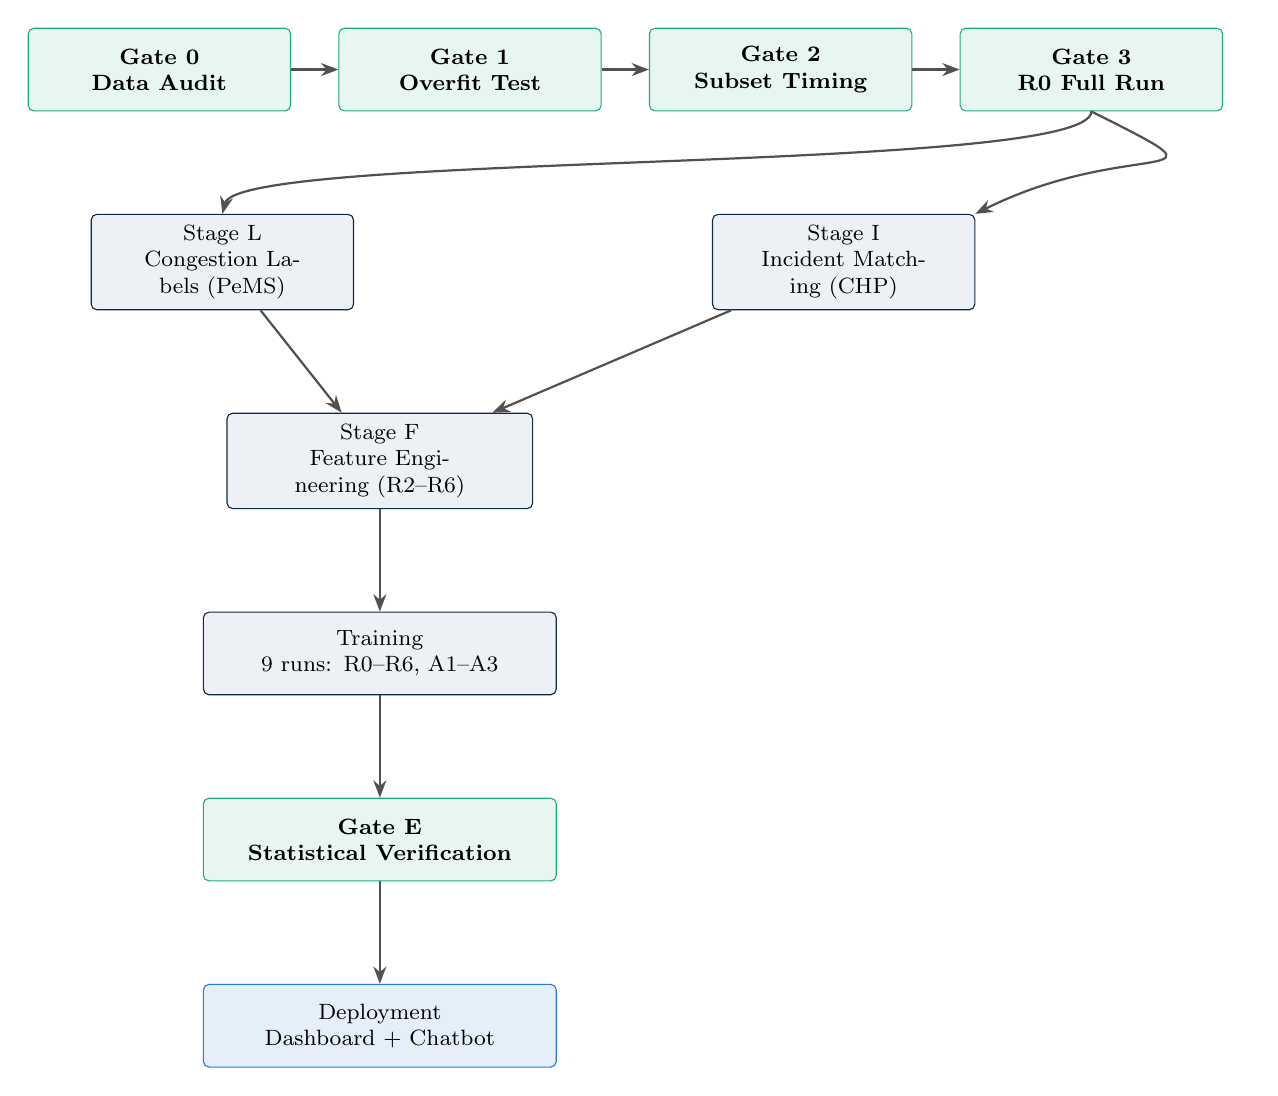
\begin{tikzpicture}[
  box/.style={draw=navy, fill=navyfill, rounded corners=2pt, text width=3.05cm, align=center, font=\footnotesize\headingfont, minimum height=1.05cm, inner sep=4pt},
  gatebox/.style={draw=accent, fill=accentfill, rounded corners=2pt, text width=3.05cm, align=center, font=\footnotesize\headingfont\bfseries, minimum height=1.05cm, inner sep=4pt},
  arr/.style={-{Stealth[length=2.2mm]}, draw=ink2, thick},
  node distance=7mm and 6mm
]
\node[gatebox] (g0) {Gate 0\\Data Audit};
\node[gatebox, right=of g0] (g1) {Gate 1\\Overfit Test};
\node[gatebox, right=of g1] (g2) {Gate 2\\Subset Timing};
\node[gatebox, right=of g2] (g3) {Gate 3\\R0 Full Run};

\node[box, below=13mm of g0, xshift=8mm] (sl) {Stage L\\Congestion Labels (PeMS)};
\node[box, below=13mm of g2, xshift=8mm] (si) {Stage I\\Incident Matching (CHP)};

\node[box, below=13mm of sl, xshift=20mm, text width=3.6cm] (sf) {Stage F\\Feature Engineering (R2--R6)};

\node[box, below=13mm of sf, text width=4.2cm] (train) {Training\\9 runs: R0--R6, A1--A3};

\node[gatebox, below=13mm of train, text width=4.2cm] (ge) {Gate E\\Statistical Verification};

\node[box, below=13mm of ge, fill=steel!12, draw=steel, text width=4.2cm] (deploy) {Deployment\\Dashboard + Chatbot};

\draw[arr] (g0) -- (g1);
\draw[arr] (g1) -- (g2);
\draw[arr] (g2) -- (g3);
\draw[arr] (g3.south) .. controls +(0,-8mm) and +(2mm,8mm) .. (sl.north);
\draw[arr] (g3.south) .. controls +(2,-10mm) and +(2,10mm) .. (si.north east);
\draw[arr] (sl) -- (sf);
\draw[arr] (si) -- (sf);
\draw[arr] (sf) -- (train);
\draw[arr] (train) -- (ge);
\draw[arr] (ge) -- (deploy);
\end{tikzpicture}
\caption{Gated development pipeline. Green boxes are hard checkpoints; each was reviewed before the
next stage began. Gate 0b (a same-day follow-up to Gate 0) is folded into Gate 0 here for space.}
\label{fig:pipeline}
\end{figure}

Every gate in Figure~\ref{fig:pipeline} produced a written, falsifiable result -- not just ``it
ran.'' The next four sections walk through what each gate actually found.

% =========================================================================
\section{Data Quality Audit (Gate 0)}

Before any model code was written, the raw LargeST data and the model's own reproduction of the
paper's published baselines were audited end to end.

\begin{itemize}
\item The paper's HL (historical-lag) baseline was \textbf{reproduced exactly}, confirming the
  local pipeline matches the published methodology bit-for-bit.
\item The timestamp index is \textbf{wall-clock, not elapsed time} -- the March 10 2:00--3:00am
  daylight-saving gap is all-zero in the data, confirmed rather than silently mishandled.
\item Zero-flow readings are \textbf{outages, not genuine zero traffic}: 94\% of zero-runs longer
  than a day coincide with clear sensor dropout signatures.
\item A hard \textbf{999 flow ceiling} appears on only 37 cells, all on 6--8 lane sensors --
  later independently confirmed against PeMS's own 5-minute archive to be genuine field
  saturation, not a pipeline artifact.
\item \textbf{5{,}049 cells imply a physically impossible rate} (over 3{,}200 vehicles per lane
  per hour), flagging lane-count metadata as suspect for a subset of sensors. On inspection, only
  one sensor (ID 1108333, metadata says 2 lanes, observed flow implies roughly 5) warranted a
  manual correction -- a plausibility fix, not a full re-audit of all 716 sensors' metadata.
\item A simple \textbf{time-of-day profile baseline} already ties the LSTM benchmark at a 2-hour
  horizon and beats it at 3 hours (test MAE 29.8 vs.\ val 21.9) -- an early signal that the LSTM
  bar, while a fair benchmark, is not an especially high one at longer horizons.
\end{itemize}

\begin{finding}
A same-day follow-up (``Gate 0b'') attributed roughly \textbf{75\% of the validation-to-test MAE
gap} to two calendar windows alone -- Thanksgiving week and December 21--31 -- with a Christmas
Day profile-baseline MAE of 127 against a median-day MAE of 23. This single finding motivated the
holiday/school-calendar feature set built later (Section~7, row R4) and is the reason the test
split's difficulty is not uniform across the quarter it covers.
\end{finding}

% =========================================================================
\section{Constructing the Congestion Label (Stage L)}

LargeST's only published quantity is flow. Congestion state -- the thing operations teams
actually respond to -- does not exist in the dataset and had to be engineered from a different
data source: raw PeMS District 11 occupancy readings, obtained independently and cross-validated
against LargeST before being trusted.

\subsection{Cross-validation against LargeST}
Before using PeMS data for anything, its flow numbers were checked against LargeST's own: 15-minute
flow matches in 99.98\% of cells (matched independently by sensor ID and wall-clock time), and
hourly aggregates correlate at 0.99998. Two asymmetries were found and are documented rather than
smoothed over: LargeST silently drops 5-minute flow readings above 999 (quietly biasing those
specific windows downward), and PeMS has genuine, non-imputed readings for 17\% of the sensor-hours
LargeST is missing entirely (86 sensors) -- meaning PeMS is a strict informational gain, not a
lossier substitute.

\subsection{Critical occupancy and the three-class label}
For each sensor, a \textbf{critical occupancy} $o_c$ is fit on training-period data only: it is
the occupancy value at which the upper envelope (95th percentile) of the flow--occupancy
relationship peaks and then declines --- the classical signature of a queue forming downstream of
that detector. Formally, with $q(o)$ the smoothed p95 flow envelope as a function of binned
occupancy $o$:
\begin{equation}
o_c = \arg\max_{o} \; q(o), \qquad \text{subject to } \min_{o' > o_c} q(o') < 0.95 \cdot q(o_c)
\end{equation}
Sensors with no observed decline after their flow peak (no congested branch was ever seen in
training data) fall back to the network median $o_c$; this affected 392 of 716 sensors, versus
278 with a directly fitted value (46 had too little data to fit at all). Given $o_c$, the hourly
label is:
\begin{equation}
\text{class}(t) = \begin{cases} \textit{congested} & \text{occupancy}(t) / o_c \ge 1.0 \\ \textit{heavy} & 0.7 \le \text{occupancy}(t)/o_c < 1.0 \\ \textit{free} & \text{occupancy}(t)/o_c < 0.7 \end{cases}
\end{equation}
and is repeated across the four 15-minute steps inside each labeled hour.

\subsection{Validation}
The label was checked five separate ways before being trusted as the training target:
\begin{itemize}
\item \textbf{Stability across splits}: class shares are consistent train/val/test (roughly
  85--88\% free, 7--9\% heavy, 5--6\% congested).
\item \textbf{Face validity}: congestion peaks at 07:00 and 16:00 on weekdays; the ten
  highest-congestion sensors by weekday-peak share are recognizable real bottlenecks (SR-78 at
  Nordahl, 78\% of weekday peak hours; SR-163 at Robinson Ave, 65\%; I-5 at Poinsettia Ln,
  60--61\%).
\item \textbf{Resolution robustness}: an independently built, genuinely 15-minute label for one
  week (Nov 4--10) agrees with the hourly-repeated label 95.7\% of the time (congested recall
  0.90, precision 0.85) -- the simplification loses some precision but is directionally sound.
\item \textbf{Spatial coherence}: congestion propagates to neighboring sensors at 12.9$\times$ the
  rate of a random sensor pair (versus 3.6$\times$ for a distance-matched control) -- it behaves
  like a real traffic queue, not sensor noise.
\end{itemize}

\begin{finding}
A na\"ive alternative -- labeling ``congested'' from flow alone, without occupancy -- was tested
and rejected. It achieves precision 0.07 and recall 0.03 against the occupancy-based label, and,
most tellingly, flags \textbf{46.8\% of Christmas Day} as congested (the occupancy-based answer:
\textbf{0.03\%}). Flow alone cannot distinguish a genuine traffic jam from a holiday with almost
no cars on the road. This is the single most important methodological decision behind the
congestion-classification half of this project.
\end{finding}

\begin{figure}[htbp]
\centering
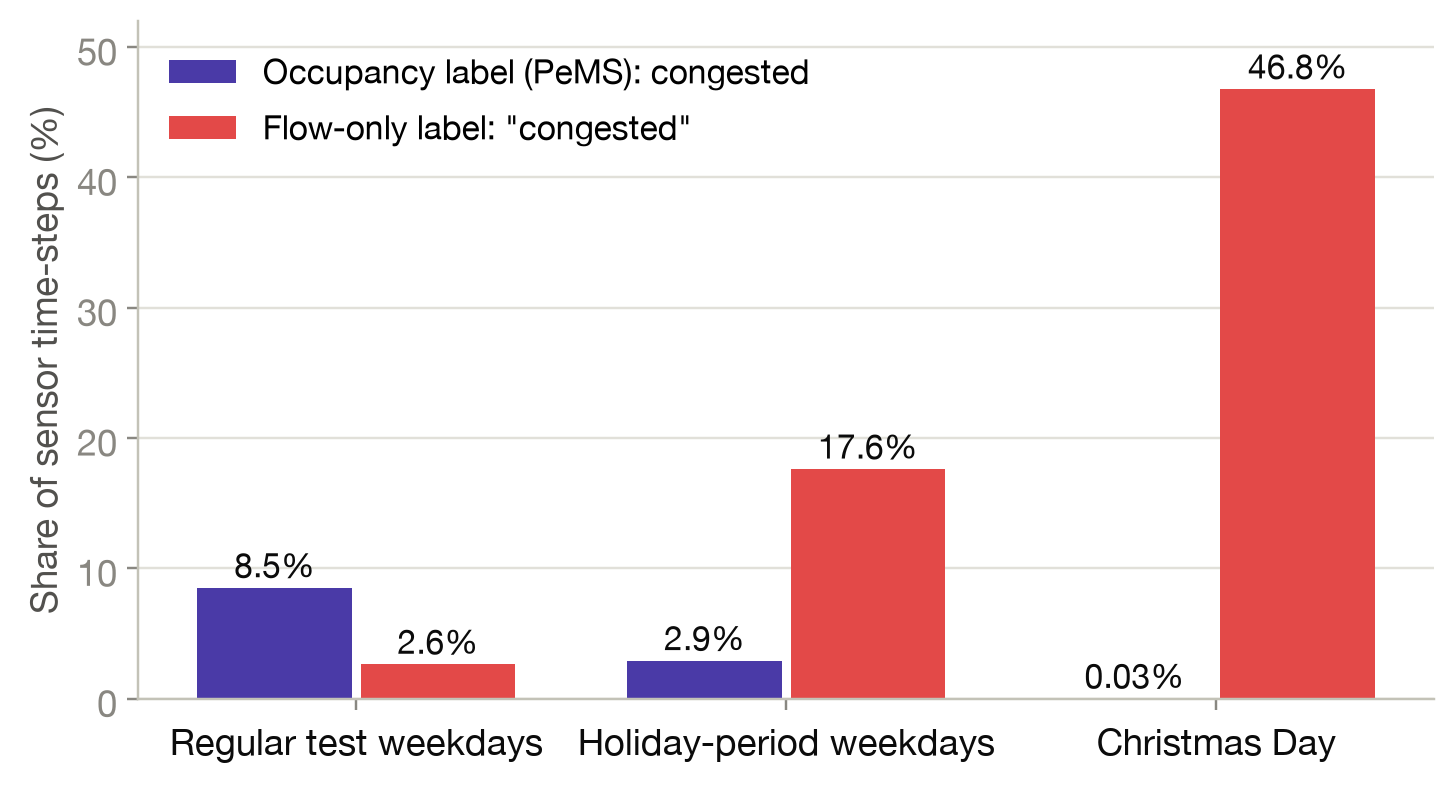
\includegraphics[width=0.72\linewidth]{labels.png}
\caption{Occupancy-based label vs.\ a flow-only proxy label, share of sensor time-steps flagged
``congested,'' by calendar period. The flow-only label inverts on holidays.}
\end{figure}

% =========================================================================
\section{Incident Intelligence (Stage I)}

49{,}198 California Highway Patrol incident records for District 11 were classified, parsed for
lanes-blocked where the free-text record allowed it (possible for 9.7\% of records; 15.5\% of
collisions specifically), and matched to the nearest sensor -- 92.6\% matched successfully.

An event-study around matched incident start times shows congestion at the nearest upstream
sensor rising by roughly \textbf{+14 percentage points} at the incident hour itself, with a
smaller \textbf{+6-point pre-rise} one hour \emph{before} the recorded start (congestion likely
contributes to the incident, not only follows it) and a decay back to baseline over about three
hours. In the test split, sensor-hours matched to an active incident show a 14.8\% congested
share versus 5.2\% for non-incident cells -- a real signal, though incident-affected cells are
only about 3\% of the test set (a point returned to in Section~11 and Section~13).

% =========================================================================
\section{Feature Engineering Program (Stage F)}

Six model configurations were trained on a strictly \textbf{cumulative} feature schedule, so that
every row's improvement (or lack of one) over the previous row isolates exactly one engineering
decision.

\begin{table}[htbp]
\centering
\small
\begin{tabular}{@{}lp{7.6cm}c@{}}
\toprule
\textbf{Run} & \textbf{Adds on top of the previous row} & \textbf{Channels} \\
\midrule
R0 & Base GWNet, LargeST's own 3 channels (flow, time-of-day, day-of-week); flow-only, single-task & 3 \\
R1 & Same inputs as R0, plus the multitask congestion head & 3 \\
R2 & Missing-data mask and causal fill for missing input flow & 4 \\
R3 & Utilization, flow-per-lane, cyclical time features, static per-sensor attributes & 33 \\
R4 & Holidays, day-before/after, holiday-period flag, school-in-session (SDUSD calendar) & 38 \\
R5 & Weather (5 San Diego ASOS stations, inverse-distance-weighted, causal) & 46 \\
R6 & CHP incident features & 50 \\
\bottomrule
\end{tabular}
\caption{Cumulative feature schedule, R0 through R6. Three further graph-ablation rows (A1--A3,
Section~10.3) reuse R0's input set to isolate the model's graph structure instead.}
\end{table}

\textbf{Missing-input fill} (from R2 onward) was chosen empirically, not by convention: four
candidate fill strategies were scored against 1\% of observed cells artificially hidden in the
validation split. ``Same weekday, last 4 weeks'' (median fill) scored best (MAE 16.9), beating a
train-only profile (21.9), a simple previous-7-days median (34.6), and zero-fill -- effectively
what LargeST does by default (255.0, i.e.\ far worse). Missing input cells are 2.28\% of the total.

\textbf{Weather} (R5) draws on NOAA/Iowa State ASOS routine METARs from five stations
(SAN/MYF/SEE/CRQ/NKX), inverse-distance-weighted onto each sensor and strictly causal --
no future weather can leak into a training window. Rain affects an uneven 7.3\% of training
steps, 0.6\% of validation steps, and 8.4\% of test steps (roughly 147 measurable hours) --
relevant context for how the weather result in Section~11 should be read.

% =========================================================================
\section{Model Architecture}

The base model is \textbf{Graph WaveNet (GWNet)}, the same architecture the LargeST paper
benchmarks (311{,}164 parameters, matching the paper's reported count), extended here with a
\textbf{multitask congestion classification head} sharing the same spatio-temporal backbone.

\begin{figure}[htbp]
\centering
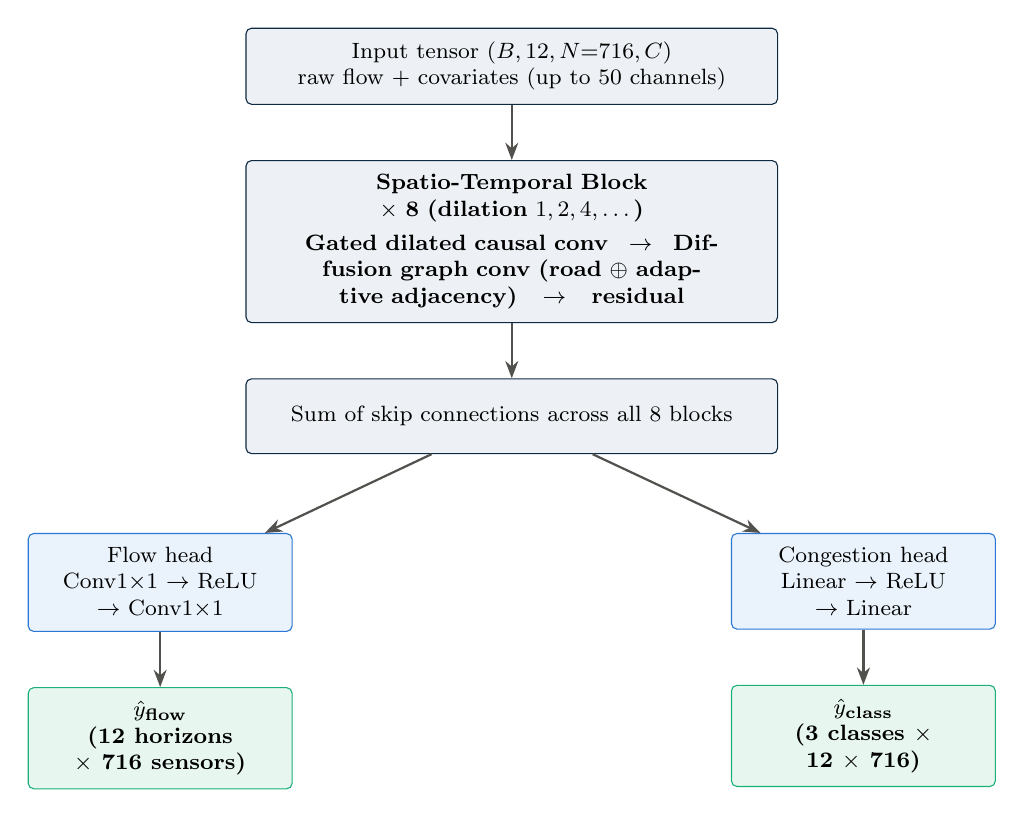
\begin{tikzpicture}[
  blk/.style={draw=navy, fill=navyfill, rounded corners=2pt, minimum height=0.95cm, align=center, font=\footnotesize\headingfont, inner sep=5pt},
  hd/.style={draw=steel, fill=steel!10, rounded corners=2pt, minimum height=0.95cm, align=center, font=\footnotesize\headingfont, inner sep=5pt},
  outbox/.style={draw=accent, fill=accentfill, rounded corners=2pt, minimum height=0.95cm, align=center, font=\footnotesize\headingfont\bfseries, inner sep=5pt},
  arr/.style={-{Stealth[length=2.2mm]}, draw=ink2, thick},
  node distance=7mm
]
\node[blk, text width=6.4cm] (input) {Input tensor $(B, 12, N{=}716, C)$\\raw flow + covariates (up to 50 channels)};
\node[blk, below=of input, text width=6.4cm, minimum height=1.6cm] (stblock) {
  \headingfont\bfseries Spatio-Temporal Block $\times$ 8 (dilation $1,2,4,\dots$) \\[3pt]
  \footnotesize Gated dilated causal conv $\;\to\;$ Diffusion graph conv (road $\oplus$ adaptive adjacency) $\;\to\;$ residual
};
\node[blk, below=of stblock, text width=6.4cm] (skip) {Sum of skip connections across all 8 blocks};
\node[hd, below left=10mm and -0.6cm of skip, text width=3.0cm] (flowhead) {Flow head\\Conv1$\times$1 $\to$ ReLU $\to$ Conv1$\times$1};
\node[hd, below right=10mm and -0.6cm of skip, text width=3.0cm] (conghead) {Congestion head\\Linear $\to$ ReLU $\to$ Linear};
\node[outbox, below=of flowhead, text width=3.0cm] (flowout) {$\hat{y}_{\text{flow}}$\\(12 horizons $\times$ 716 sensors)};
\node[outbox, below=of conghead, text width=3.0cm] (classout) {$\hat{y}_{\text{class}}$\\(3 classes $\times$ 12 $\times$ 716)};
\draw[arr] (input) -- (stblock);
\draw[arr] (stblock) -- (skip);
\draw[arr] (skip) -- (flowhead);
\draw[arr] (skip) -- (conghead);
\draw[arr] (flowhead) -- (flowout);
\draw[arr] (conghead) -- (classout);
\end{tikzpicture}
\caption{GWNet backbone with the multitask congestion head. The classification head branches off
the same shared skip-connection representation the flow head reads from -- both tasks see
identical spatio-temporal features, differing only in their final projection.}
\label{fig:arch}
\end{figure}

\subsection{Core mechanics}

Each spatio-temporal block combines a \textbf{gated dilated causal convolution} (the WaveNet
half) with a \textbf{diffusion graph convolution} (the spatial half):
\begin{align}
h &= \tanh(W_f * x) \odot \sigma(W_g * x) \\
Z &= \sum_{k=0}^{K} \Big( P_f^{k}\, h\, \Theta_{f,k} \;+\; P_b^{k}\, h\, \Theta_{b,k} \Big)
\end{align}
where $*$ is a dilated causal convolution along the time axis, $\odot$ is element-wise product,
and $P_f, P_b$ are the forward and backward random-walk transition matrices derived from an
adjacency $A$. GWNet's key architectural contribution is that $A$ is not fixed to the physical
road network alone -- it also learns a data-driven \textbf{adaptive adjacency}:
\begin{equation}
A_{\text{adp}} = \text{softmax}\big(\text{ReLU}(E_1 E_2^{\top})\big)
\end{equation}
from two learnable node-embedding matrices $E_1, E_2 \in \mathbb{R}^{716 \times 10}$ (14{,}320
parameters total) -- letting the model discover statistical relationships between sensors the
physical road graph does not encode (for instance, correlated but non-adjacent corridors).
Section~10.3 quantifies exactly how much each adjacency source contributes.

\begin{sowhat}
One architectural quirk was identified and is reported for completeness, not as a defect: the
base GWNet's final graph-convolution/batch-norm layer (7{,}264 of the 311{,}164 parameters) never
receives gradient, because the network's output is read from the skip connections \emph{before}
that final layer. This does not affect correctness -- the paper's own published parameter count
includes these unused parameters too -- but it is worth knowing before reading too much into a
raw parameter count as a proxy for effective model capacity.
\end{sowhat}

\subsection{Loss function}

The flow task uses LargeST's own \textbf{masked MAE} -- cells where the true label is exactly
zero (a missing-data sentinel, not genuine zero flow; see Section~4) are excluded from the loss
and from every reported metric:
\begin{equation}
\mathcal{L}_{\text{flow}} = \frac{\sum_i \mathbb{1}[y_i \neq 0]\,\lvert \hat{y}_i - y_i \rvert}{\sum_i \mathbb{1}[y_i \neq 0]}
\end{equation}
The congestion task uses a class-weighted cross-entropy, with weights set to the inverse square
root of each class's training-set frequency ($w_c = 1/\sqrt{f_c}$) to counteract the roughly
17:1 imbalance between the free and congested classes. The two objectives are combined as
\begin{equation}
\mathcal{L} = \mathcal{L}_{\text{flow}} + \lambda\, \mathcal{L}_{\text{class}}, \qquad \lambda = 15
\end{equation}
$\lambda$ was fixed at 15 across every multitask run (R1 through R6) rather than tuned per row, so
that the feature-ablation comparisons in Section~10 isolate the effect of the input features
alone.

% =========================================================================
\section{Training Protocol and Readiness Gates}

Three gates preceded any full training run, each designed to catch a specific class of failure
cheaply before committing laptop-hours to it.

\begin{description}[leftmargin=0pt, style=nextline]
\item[\gate{Gate 1 -- Overfit Test.}] A full 100-window memorization run is computationally
  infeasible for this model (100 windows $\times$ 12 horizons $\times$ 716 sensors implies 859{,}000
  targets against roughly 304{,}000 trainable parameters). The actual test was a 4-window,
  full-batch memorization run, which must drive training loss below 10\% of its starting value
  and keep falling -- passed on the M2 (loss fell from 152.4 to 4.6) -- backed by the 100-window
  run as a supplementary sanity curve, not the primary pass/fail criterion.
\item[\gate{Gate 2 -- Subset Timing.}] Five epochs on a 60-day data subset, intended to validate
  throughput and surface obvious training-loop bugs cheaply. It failed one of its stated criteria
  (beating the time-of-day profile baseline at horizons 1--3) -- a result later shown by Gate 3
  to be simple undertraining at 5 epochs, not a flaw in the setup.
\item[\gate{Gate 3 -- First 25\% of R0.}] Three epochs on the \emph{full} dataset. Validation-subset
  MAE fell from 43.4 to 26.5, beating both the historical-lag and profile baselines at horizons
  1--3 (the profile baseline remained ahead at horizon $\ge 4$, as expected at only 3 epochs).
  This gate passed and fixed the final training recipe used for every subsequent run: \textbf{16
  epochs}, seed 2023, a warmup $\to$ constant $\to$ cosine-decay learning-rate schedule (the
  decay covering the final 30\% of training).
\end{description}

Nine runs followed this exact recipe: R0 through R6 (the feature ablation, Section~7) and A1
through A3 (the graph ablation, Section~10.3). They were executed in a fixed dependency order
--- R2 $\to$ A2 $\to$ R1 $\to$ R3 $\to$ R4 $\to$ R5 $\to$ R6, with A1/A3 run earlier --- via a
detached, resumable queue script, completing over roughly 65 hours of wall-clock time between
2026-09-15 and 2026-09-18.

% =========================================================================
\section{Results}

All figures in this section are \textbf{test-set} averages across all 12 forecast horizons (15
minutes to 3 hours ahead) unless stated otherwise.

\subsection{Headline performance}

\begin{table}[htbp]
\centering
\begin{tabular}{@{}lccc@{}}
\toprule
\textbf{Model} & \textbf{avg MAE} & \textbf{avg RMSE} & \textbf{avg MAPE} \\
\midrule
HL (historical lag, paper) & 60.79 & -- & -- \\
Time-of-day profile (ours) & 29.8 & -- & -- \\
LSTM (client baseline) & 26.35 & -- & -- \\
GWNet (paper, flow-only, $\sim$80 epochs) & 17.74 & -- & -- \\
\rowcolor{accentfill}\textbf{R4 (this project)} & \textbf{18.56} & \textbf{30.97} & \textbf{12.25\%} \\
\bottomrule
\end{tabular}
\caption{Headline comparison. R4 is 29.6\% below the client's LSTM baseline and within 4.6\% of the
paper's own flow-only GWNet trained under a far larger compute budget.}
\end{table}

\subsection{Full feature-ablation table}

\begin{table}[htbp]
\centering
\small
\begin{tabular}{@{}lccccc@{}}
\toprule
\textbf{Run} & \textbf{avg MAE} & \textbf{avg RMSE} & \textbf{avg MAPE} & \textbf{macro-F1} & \textbf{F1: free / heavy / congested} \\
\midrule
R0 & 20.35 & 33.48 & 13.40\% & -- & -- \\
R1 & 20.41 & 33.70 & 13.65\% & 0.768 & -- \\
R2 & 20.39 & 33.63 & 13.81\% & 0.769 & -- \\
R3 & 18.90 & 31.60 & 12.63\% & 0.780 & -- \\
\rowcolor{accentfill} R4 & \textbf{18.56} & \textbf{30.97} & \textbf{12.25\%} & \textbf{0.790} & 0.975 / 0.665 / 0.730 \\
R5 & 18.64 & 31.03 & 12.27\% & 0.787 & -- \\
R6 & 18.70 & 31.22 & 12.26\% & 0.787 & -- \\
\bottomrule
\end{tabular}
\caption{Cumulative feature ablation, test set. R4 is both the lowest-error and highest-F1 row.}
\end{table}

\begin{figure}[htbp]
\centering
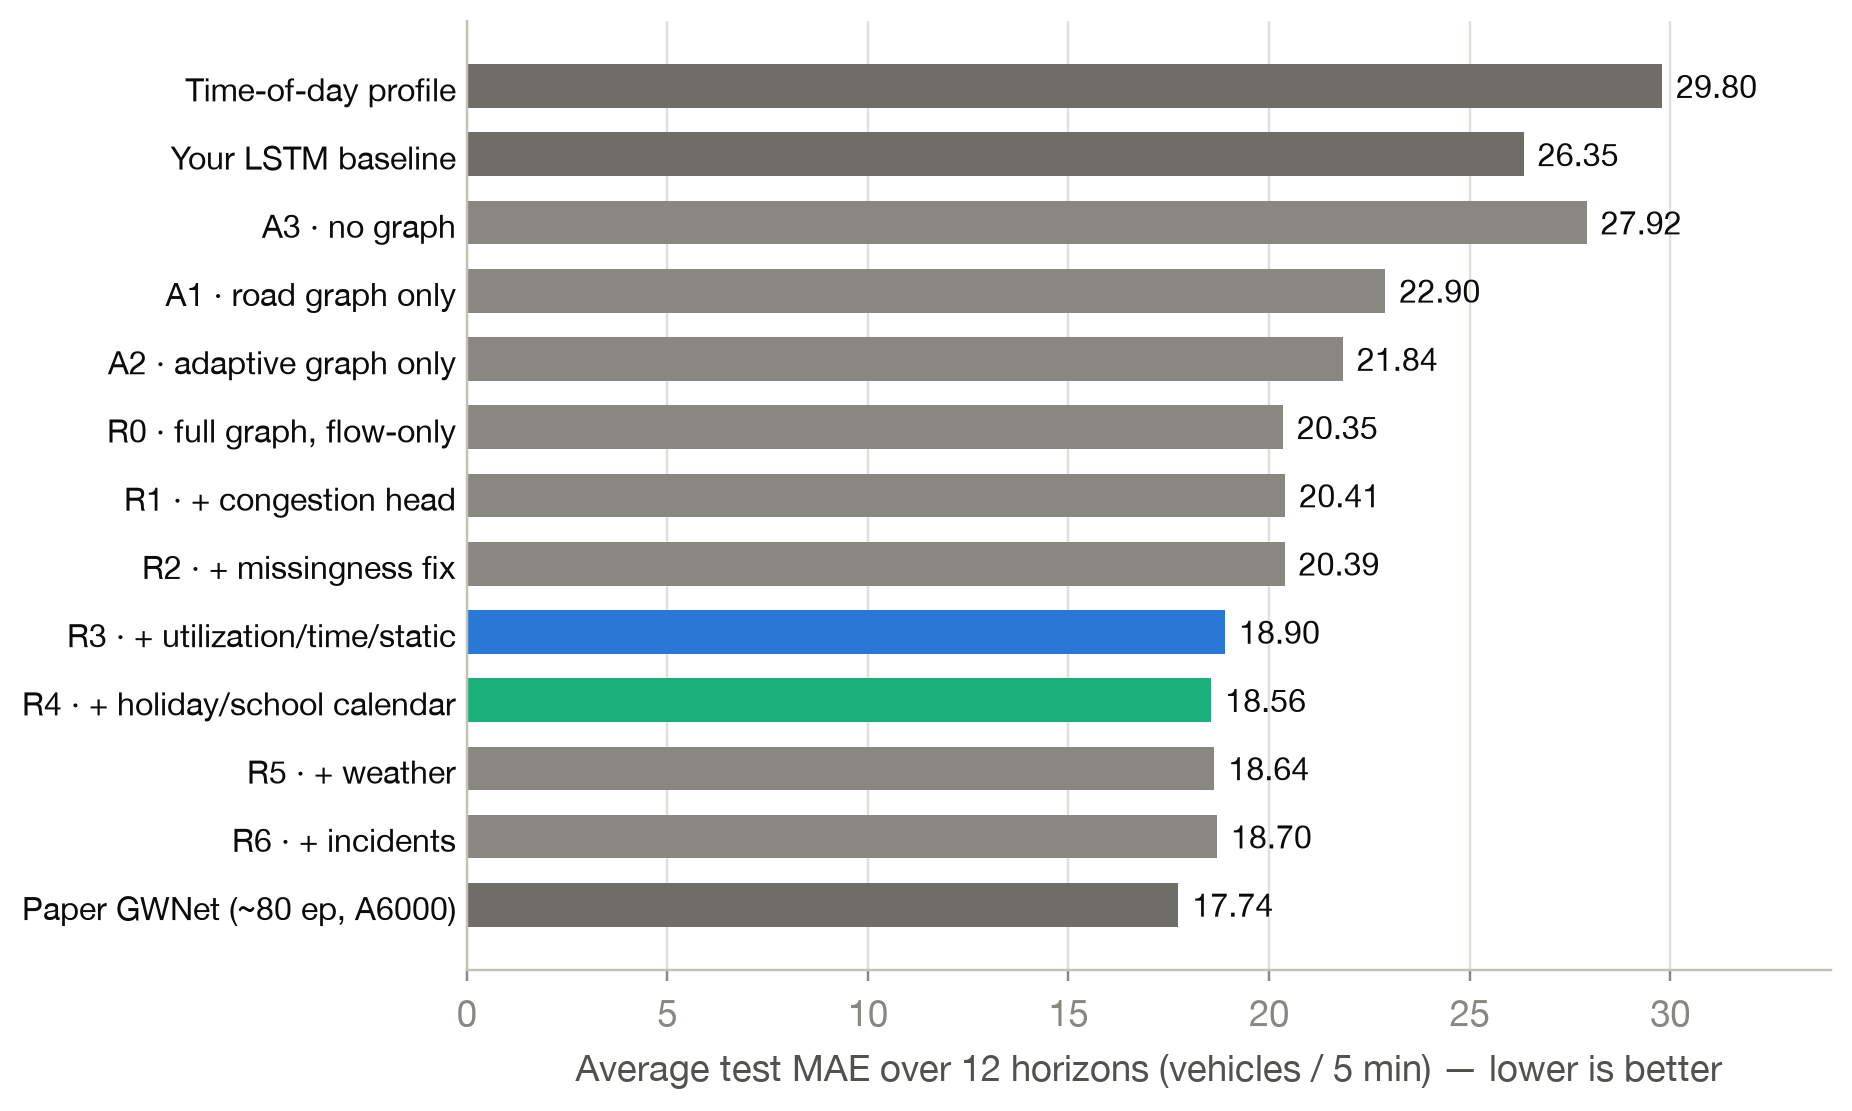
\includegraphics[width=0.92\linewidth]{ablation_all.png}
\caption{Average test MAE, every run and baseline. R3 and R4 (highlighted) are the two rows a
statistical test confirms as real improvements -- see Section~11.}
\end{figure}

\subsection{Graph ablation: how much does the graph structure matter?}

Four configurations, all trained on R0's input set, isolate the contribution of GWNet's two
adjacency sources (Section~8.1).

\begin{figure}[htbp]
\centering
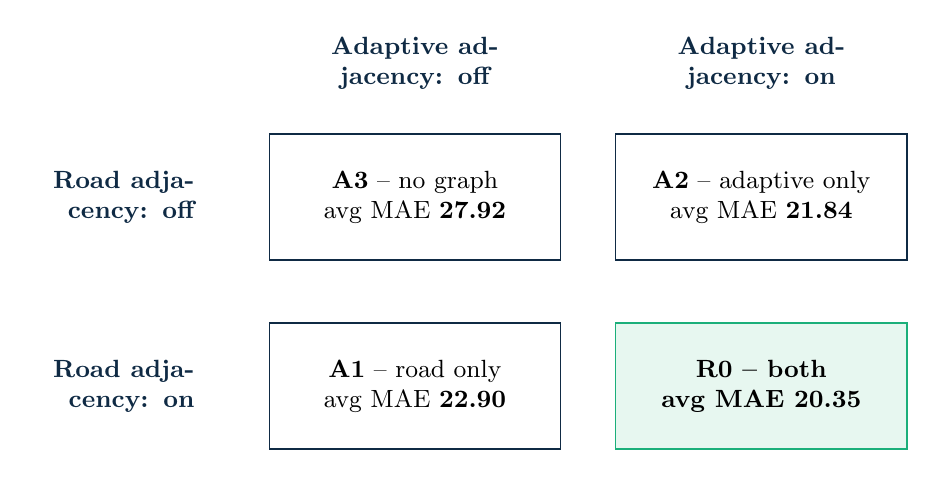
\begin{tikzpicture}[
  cell/.style={draw=navy, minimum width=3.7cm, minimum height=1.6cm, text width=3.3cm, align=center, font=\small\headingfont, inner sep=4pt},
  best/.style={draw=accent, fill=accentfill, minimum width=3.7cm, minimum height=1.6cm, text width=3.3cm, align=center, font=\small\headingfont\bfseries, inner sep=4pt},
  colhdr/.style={font=\small\headingfont\bfseries, text=navy, text width=3.7cm, align=center},
  rowhdr/.style={font=\small\headingfont\bfseries, text=navy, text width=2.0cm, align=right},
  xcol1/.style={xshift=2.2cm}, xcol2/.style={xshift=6.6cm},
]
\node[colhdr] (c1) at (2.2,2.1) {Adaptive adjacency: off};
\node[colhdr] (c2) at (6.6,2.1) {Adaptive adjacency: on};
\node[rowhdr] (r1) at (-1.6,0.4) {Road adjacency: off};
\node[rowhdr] (r2) at (-1.6,-2.0) {Road adjacency: on};
\node[cell] at (2.2,0.4) {\textbf{A3} -- no graph\\avg MAE \textbf{27.92}};
\node[cell] at (6.6,0.4) {\textbf{A2} -- adaptive only\\avg MAE \textbf{21.84}};
\node[cell] at (2.2,-2.0) {\textbf{A1} -- road only\\avg MAE \textbf{22.90}};
\node[best] at (6.6,-2.0) {\textbf{R0} -- both\\avg MAE \textbf{20.35}};
\end{tikzpicture}
\caption{Graph ablation, 2$\times$2. The two adjacency sources are complementary, not redundant --
using both beats either alone.}
\label{fig:graph2x2}
\end{figure}

\begin{finding}
Adaptive adjacency alone recovers roughly \textbf{80\%} of the full model's improvement over
no-graph (21.84 vs.\ 27.92 vs.\ 20.35); road adjacency alone recovers roughly \textbf{66\%}
(22.90). Both together are better than either alone -- confirmed as a statistically real gap in
Section~11 -- meaning the model is not simply re-deriving the road network from data: it is
learning something the physical graph does not encode.
\end{finding}

\begin{figure}[htbp]
\centering
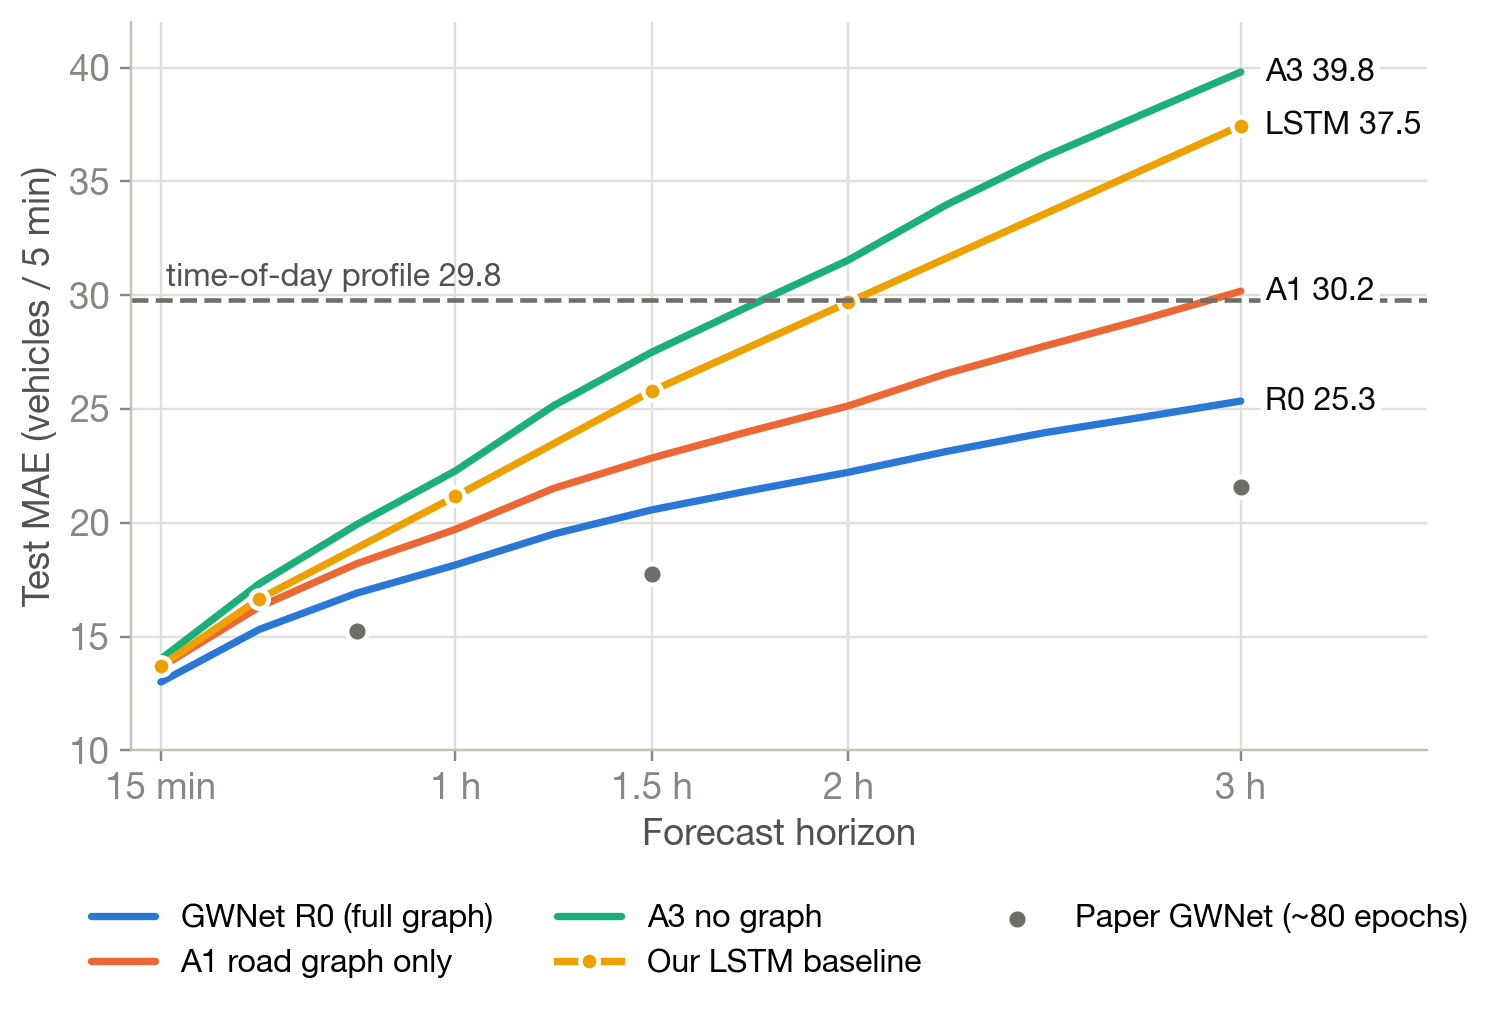
\includegraphics[width=0.85\linewidth]{horizon.png}
\caption{Test MAE by forecast horizon, graph-ablation rows against both baselines. The gap
between configurations widens, not narrows, at longer horizons.}
\end{figure}

\subsection{Classification performance in context}

\begin{table}[htbp]
\centering
\footnotesize
\begin{tabular}{@{}p{5.6cm}cccc@{}}
\toprule
\textbf{Baseline / model} & \textbf{macro-F1} & \textbf{free} & \textbf{heavy} & \textbf{congested} \\
 & & \multicolumn{3}{c}{\scriptsize (recall, except R4 which reports F1)} \\
\midrule
Persistence (hold last known class) & 0.656 & 0.951 & 0.496 & 0.522 \\
Profile-class (train-fitted majority per sensor/slot/day-type) & 0.761 & 0.969 & 0.656 & 0.667 \\
\rowcolor{accentfill}\textbf{R4} & \textbf{0.790} & 0.975 & 0.665 & 0.730 \\
\bottomrule
\end{tabular}
\caption{R4 against the two strongest available classification baselines. The profile-class
baseline is a strong bar precisely because congestion is highly time-of-day-dependent -- R4
still improves meaningfully on the operationally critical heavy/congested classes.}
\end{table}

\subsection{Stratified diagnostics}

Every model was also evaluated on eight overlapping subsets of the test set -- rain vs.\ dry,
incident-affected vs.\ not, peak vs.\ off-peak, holiday-period vs.\ not, and each true congestion
class -- to check whether the aggregate number hides an important asymmetry. It does.

\begin{table}[htbp]
\centering
\scriptsize
\setlength{\tabcolsep}{3.4pt}
\begin{tabular}{@{}lcccccccccccc@{}}
\toprule
\textbf{Run} & overall & rain & dry & incident & non-incid. & peak & off-peak & holiday & non-hol. & free & heavy & congested \\
\midrule
R0 & 20.35 & 28.17 & 19.64 & 30.09 & 20.03 & 32.07 & 17.27 & 24.74 & 19.74 & 17.46 & 30.09 & 44.33 \\
A1 & 22.90 & 29.87 & 22.27 & 32.69 & 22.59 & 36.02 & 19.46 & 26.62 & 22.38 & 19.94 & 35.18 & 49.46 \\
A2 & 21.84 & 29.83 & 21.12 & 31.83 & 21.52 & 35.24 & 18.32 & 26.06 & 21.25 & 18.70 & 32.75 & 47.88 \\
A3 & 27.92 & 32.42 & 27.51 & 38.20 & 27.59 & 45.57 & 23.28 & 28.76 & 27.80 & 24.25 & 46.58 & 61.97 \\
R1 & 20.41 & 28.37 & 19.68 & 30.21 & 20.09 & 32.14 & 17.33 & 25.39 & 19.71 & 17.60 & 29.99 & 42.78 \\
R2 & 20.39 & 29.23 & 19.59 & 30.02 & 20.08 & 32.69 & 17.16 & 25.88 & 19.62 & 17.68 & 29.37 & 42.50 \\
R3 & 18.90 & 26.66 & 18.20 & 28.76 & 18.59 & 29.81 & 16.04 & 24.68 & 18.10 & 16.04 & 27.45 & 40.87 \\
\rowcolor{accentfill}R4 & \textbf{18.56} & \textbf{26.15} & \textbf{17.87} & \textbf{28.40} & \textbf{18.24} & \textbf{29.21} & \textbf{15.76} & \textbf{23.83} & \textbf{17.82} & \textbf{15.65} & \textbf{27.40} & \textbf{40.60} \\
R5 & 18.64 & 25.79 & 17.99 & 28.42 & 18.32 & 29.30 & 15.84 & 23.87 & 17.91 & 15.76 & 27.11 & 40.29 \\
R6 & 18.70 & 26.10 & 18.03 & 28.53 & 18.39 & 29.49 & 15.87 & 24.02 & 17.96 & 15.81 & 27.29 & 40.52 \\
\bottomrule
\end{tabular}
\caption{Stratified test flow-MAE, every run $\times$ every stratum. Mask coverage: rain 8.30\%,
incident 3.07\%, peak 20.76\%, holiday-period 12.32\%, true free/heavy/congested 74.58\% / 6.21\%
/ 4.67\% of test sensor-timesteps.}
\label{tab:strat}
\end{table}

% =========================================================================
\section{Statistical Verification (Gate E)}

A row-to-row improvement in Section~10 could, in principle, be sampling noise rather than a real
effect of the feature or architecture change behind it. Gate E answers this directly with a
\textbf{paired, day-block bootstrap}: the 74 distinct calendar days the test set's forecast
origins fall on are resampled with replacement 1{,}000 times; for each resample, the MAE delta
between two models is recomputed from only the resampled days, giving an empirical distribution
of the delta and a 95\% confidence interval by the percentile method:
\begin{equation}
\text{CI}_{95\%} = \big[\, Q_{2.5}(\Delta^{*}),\; Q_{97.5}(\Delta^{*}) \,\big], \qquad
\Delta^{*}_b = \overline{\text{MAE}}_{\text{to}}(D_b) - \overline{\text{MAE}}_{\text{from}}(D_b)
\end{equation}
where $D_b$ is the $b$-th resample of test days (with replacement) and $\overline{\text{MAE}}(D_b)$
is that model's MAE recomputed over only the windows originating on days in $D_b$. Blocking by
day (rather than treating every 15-minute window as an independent sample) accounts for the fact
that forecast errors on nearby windows within the same day are correlated, not independent draws.

\begin{figure}[htbp]
\centering
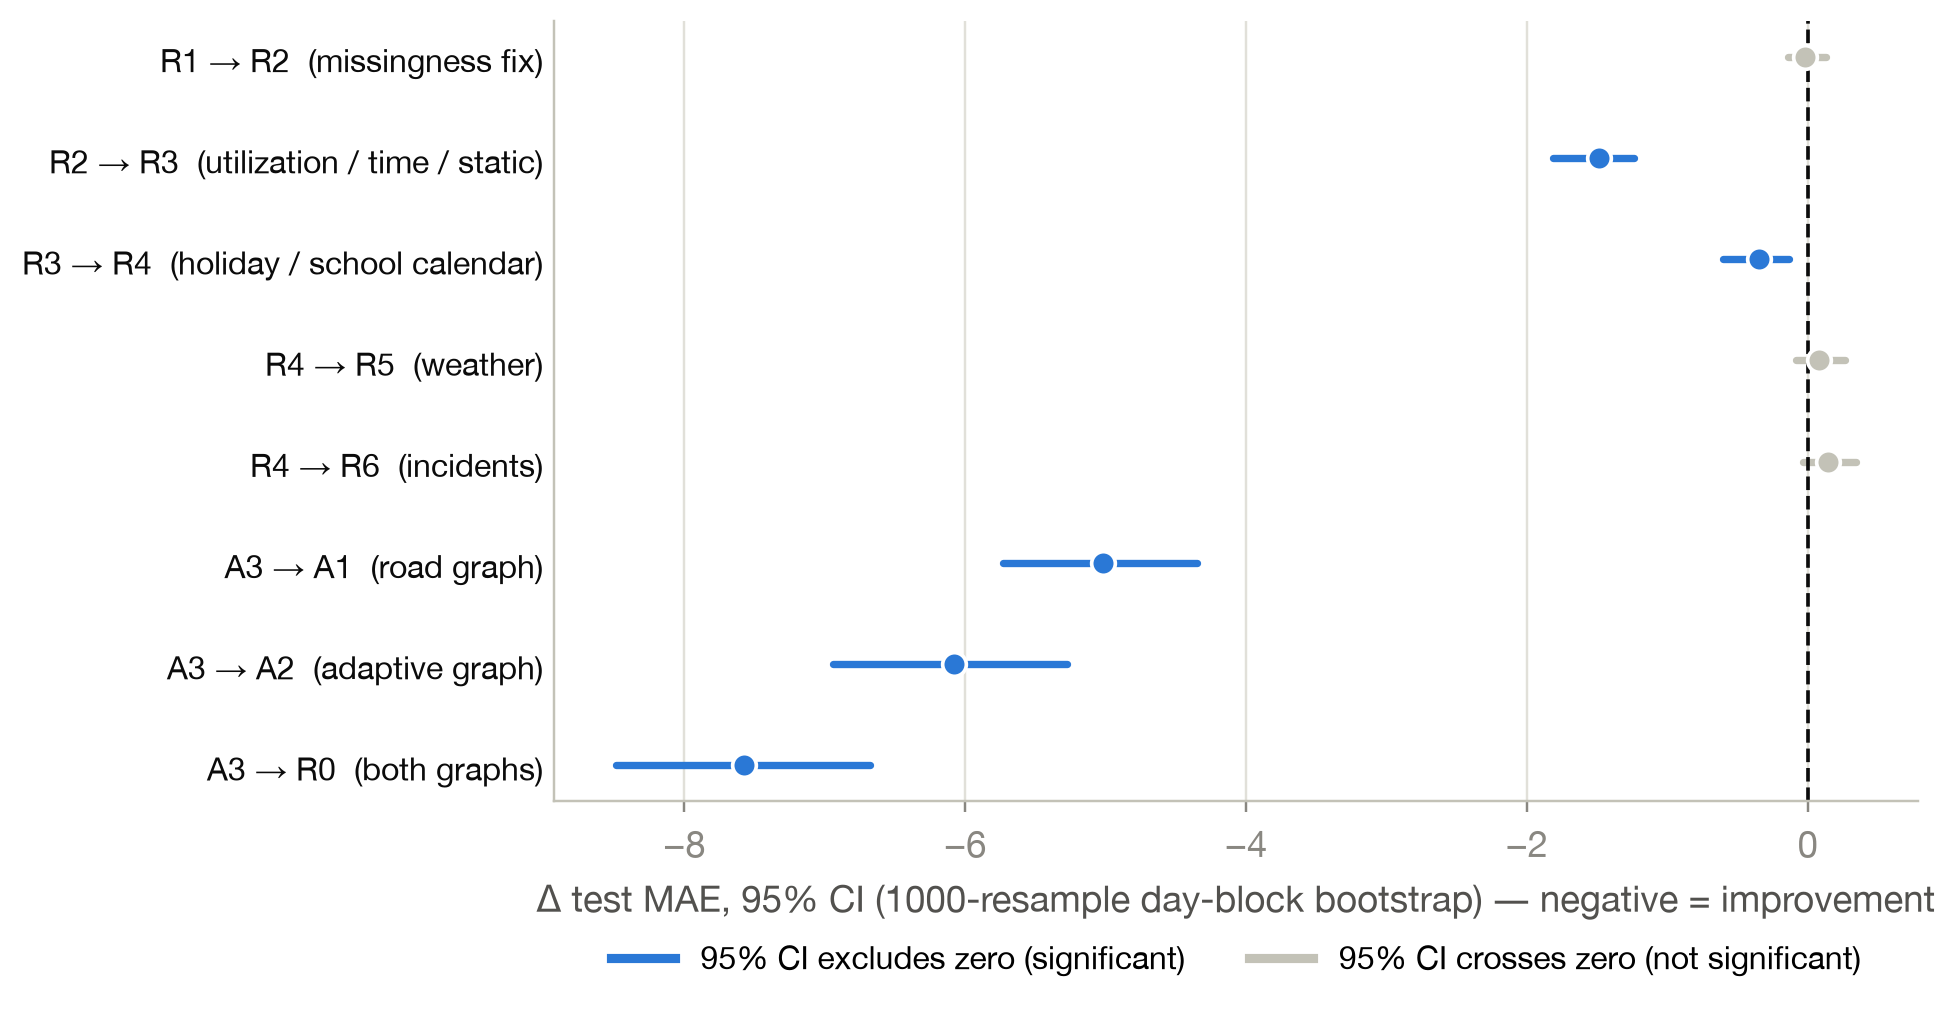
\includegraphics[width=0.92\linewidth]{bootstrap_forest.png}
\caption{Bootstrap 95\% confidence intervals on eight row-to-row deltas. A blue interval excludes
zero (statistically real); a gray interval crosses it (not distinguishable from noise).}
\label{fig:forest}
\end{figure}

\begin{table}[htbp]
\centering
\small
\begin{tabular}{@{}lccc@{}}
\toprule
\textbf{Comparison} & $\boldsymbol{\Delta}$\textbf{MAE} & \textbf{95\% CI} & \textbf{Significant?} \\
\midrule
R1 $\to$ R2 (missingness fix) & $-0.018$ & $[-0.140,\ 0.135]$ & No \\
R2 $\to$ R3 (utilization / time / static) & $-1.486$ & $[-1.811,\ -1.233]$ & \textbf{Yes} \\
R3 $\to$ R4 (holiday / school calendar) & $-0.346$ & $[-0.604,\ -0.131]$ & \textbf{Yes} \\
R4 $\to$ R5 (weather) & $+0.080$ & $[-0.082,\ 0.264]$ & No \\
R4 $\to$ R6 (incidents) & $+0.144$ & $[-0.029,\ 0.343]$ & No \\
A3 $\to$ A1 (road graph) & $-5.020$ & $[-5.732,\ -4.345]$ & \textbf{Yes} \\
A3 $\to$ A2 (adaptive graph) & $-6.079$ & $[-6.939,\ -5.274]$ & \textbf{Yes} \\
A3 $\to$ R0 (both graphs) & $-7.574$ & $[-8.488,\ -6.680]$ & \textbf{Yes} \\
\bottomrule
\end{tabular}
\caption{Gate E bootstrap results, 1{,}000 resamples over 74 test-origin days.}
\end{table}

\begin{finding}
\textbf{R4 is the statistically best model, not merely the lowest-MAE one.} The R2$\to$R3 and
R3$\to$R4 improvements are real by this test; R4$\to$R5 and R4$\to$R6 are not. But the aggregate
result for R5 and R6 hides an asymmetry visible directly in Table~\ref{tab:strat}: inside the
\emph{rain} stratum specifically, R5 improves on R4 (26.15 $\to$ 25.79 MAE) -- a genuine, if
minor, effect masked in aggregate only because rain covers just 8.3\% of test cells. Inside the
\emph{incident} stratum specifically, R6 does \emph{not} improve on R4 (28.40 $\to$ 28.53, worse)
-- unlike weather, the incident feature shows no localized benefit even where incidents are
active, which is reported here as a genuine negative result rather than quietly dropped.
\end{finding}

\begin{sowhat}
The decision taken at this gate was to \textbf{ship R4} as the model behind the dashboard, the
chatbot, and the final review deck -- not R6, despite R6 having strictly more engineered
features. More features are not automatically better; the bootstrap is what separates a genuine
improvement from noise dressed up as one, and that discipline is what this project is
recommending as a general practice, independent of this specific dataset.
\end{sowhat}

% =========================================================================
\section{Key Findings and Recommendations}

\begin{enumerate}
\item \textbf{Ship R4, not R6.} Every additional engineered feature increases system complexity
  and maintenance burden. R6 has the most features and is not the best model by a statistical
  test -- a reminder to gate feature additions on evidence, not on effort invested.
\item \textbf{Congestion labels built from occupancy, not flow, are a prerequisite for any
  congestion-classification product on this kind of sensor network.} The flow-only proxy's
  46.8\%-of-Christmas-Day failure mode would have silently corrupted any downstream alerting or
  reporting built on it.
\item \textbf{Both graph sources earn their place.} The learned adaptive adjacency is not simply
  rediscovering the physical road network -- it recovers more of the total graph benefit alone
  (80\%) than the road graph does alone (66\%), and using both is better than either. For a
  network expansion or a new region without a clean road-adjacency file, this suggests the
  adaptive mechanism alone is already most of the value.
\item \textbf{Weather is a real, narrow-scope win; incidents currently are not.} Both are
  reasonable hypotheses to test on any traffic network; this project's evidence is that only one
  of the two paid off here, and by how much (Section~11) -- a result that should inform, not
  discourage, testing the same features on a larger or wetter dataset where the strata would
  carry more weight.
\item \textbf{Holiday-period behavior is disproportionately represented in this test window} and
  disproportionately hard to predict (Section~4, Section~13) -- a structural property of a
  Q4-only test split that any production deployment on a similar calendar footprint should plan
  around, e.g.\ with holiday-specific model variants or wider training data coverage.
\end{enumerate}

% =========================================================================
\section{Limitations}

\begin{riskbox}
\textbf{Congestion is measured, not observed directly.} The label is derived from PeMS
occupancy -- itself an inferred signal from per-lane loop-detector on-time, not a direct queue
measurement. Thresholds are fitted per sensor and validated five ways (Section~5), but remain a
modeling choice.
\end{riskbox}

\begin{riskbox}
\textbf{PeMS occupancy is itself partly imputed.} Roughly 10\% of underlying sensor-hours are
below 50\% observed and were excluded from \emph{label fitting}; the \emph{flow} series those
hours feed via LargeST was not separately filtered.
\end{riskbox}

\begin{riskbox}
\textbf{Test-only holidays.} Thanksgiving and December 21--31 appear only in the test split,
never in training or validation. The model must generalize holiday behavior from smaller
training-set analogues (New Year's, Memorial Day, July 4th) -- R4's calendar-feature gain is real
on this split, but the largest test-period anomalies are exactly the days with the least similar
training exposure.
\end{riskbox}

\begin{riskbox}
\textbf{Single seed, fixed epoch budget.} Every run used one seed (2023) and 16 epochs, against
the paper's roughly 80-epoch, data-center training budget. The bootstrap in Section~11 quantifies
\emph{test-sampling} uncertainty only, not \emph{training-seed} uncertainty, which was not
measured given the available compute.
\end{riskbox}

\begin{riskbox}
\textbf{Weather and incident coverage are limited by what actually occurred in the test
period} -- about 147 hours of measurable rain, about 3\% incident-affected cells. Real effects,
on a comparatively small slice of the data; the R5/R6 stratified findings in Section~11 should be
read as suggestive, not as tightly bounded estimates.
\end{riskbox}

\begin{riskbox}
\textbf{One hand-corrected sensor.} Lane count for sensor 1108333 was corrected manually
(metadata said 2 lanes; observed flow implies roughly 5) -- a targeted plausibility fix, not a
systematic re-audit of all 716 sensors' metadata.
\end{riskbox}

% =========================================================================
\section{Solution Deployment: Dashboard and Chatbot}

The final deliverable pairs R4 with a working analytics tool, built to run entirely locally --
a deliberate choice after weighing a hosted deployment's free-tier resource limits against the
timeline to the final review.

\begin{figure}[htbp]
\centering
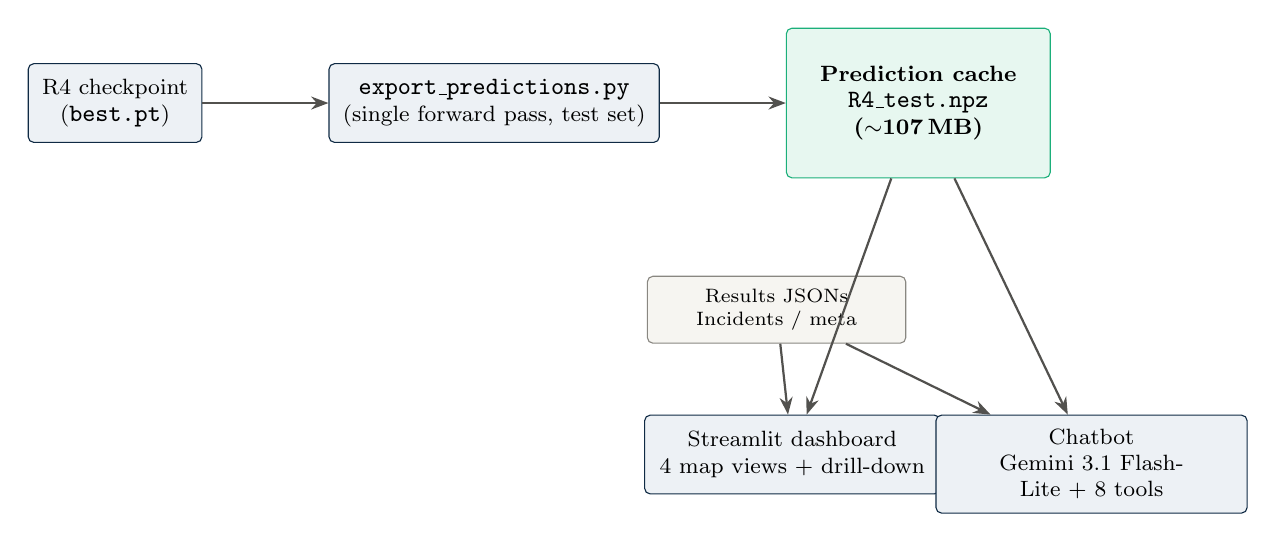
\begin{tikzpicture}[
  blk/.style={draw=navy, fill=navyfill, rounded corners=2pt, minimum height=1.0cm, align=center, font=\footnotesize\headingfont, inner sep=5pt},
  data/.style={draw=muted, fill=lightbg, rounded corners=2pt, minimum height=0.85cm, align=center, font=\scriptsize\headingfont, inner sep=4pt},
  outbox/.style={draw=accent, fill=accentfill, rounded corners=2pt, minimum height=1.0cm, align=center, font=\footnotesize\headingfont\bfseries, inner sep=5pt},
  arr/.style={-{Stealth[length=2.2mm]}, draw=ink2, thick},
]
\node[blk] (ckpt) {R4 checkpoint\\(\code{best.pt})};
\node[blk, right=16mm of ckpt] (export) {\code{export\_predictions.py}\\(single forward pass, test set)};
\node[outbox, right=16mm of export, text width=3.0cm, minimum height=1.9cm] (cache) {Prediction cache\\\code{R4\_test.npz}\\($\sim$107\,MB)};
\node[blk, below=30mm of cache, xshift=-1.6cm, text width=3.4cm] (dash) {Streamlit dashboard\\4 map views + drill-down};
\node[blk, below=30mm of cache, xshift=2.2cm, text width=3.6cm] (bot) {Chatbot\\Gemini 3.1 Flash-Lite + 8 tools};
\node[data, above=9mm of dash, xshift=-0.2cm, text width=3.0cm] (side1) {Results JSONs\\Incidents / meta};
\draw[arr] (ckpt) -- (export);
\draw[arr] (export) -- (cache);
\draw[arr] (cache) -- (dash);
\draw[arr] (cache) -- (bot);
\draw[arr] (side1) -- (dash);
\draw[arr] (side1) -- (bot);
\end{tikzpicture}
\caption{Dashboard and chatbot data flow. Neither surface requires PyTorch at runtime -- only the
prediction cache and small JSON/metadata files, which keeps the running application lightweight.}
\end{figure}

\subsection{Map views and live KPIs}
Four synchronized map views, all driven by the same sidebar date / time / horizon controls:
predicted congestion state, predicted-vs-actual flow (color = signed \% error), an incident
overlay, and an error-magnitude view for model-quality diagnosis separate from the raw
comparison -- plus a sensor drill-down showing actual-vs-predicted flow across a chosen day at
multiple horizons. A \textbf{KPI header row} (network average predicted flow, \% congested/heavy,
active CHP incidents, this window's MAE against the model's overall average) recomputes live off
whatever the sidebar is set to; an \textbf{ops watchlist} ranks sensors congested-first for the
current slot; an \textbf{auto-play} control steps the time slider forward automatically; and a
\textbf{model-performance view} brings the ablation chart, the Gate E bootstrap forest plot, and
the Section~10--11 findings directly into the app as FINDING/LIMITATION callouts.

\begin{figure}[htbp]
\centering
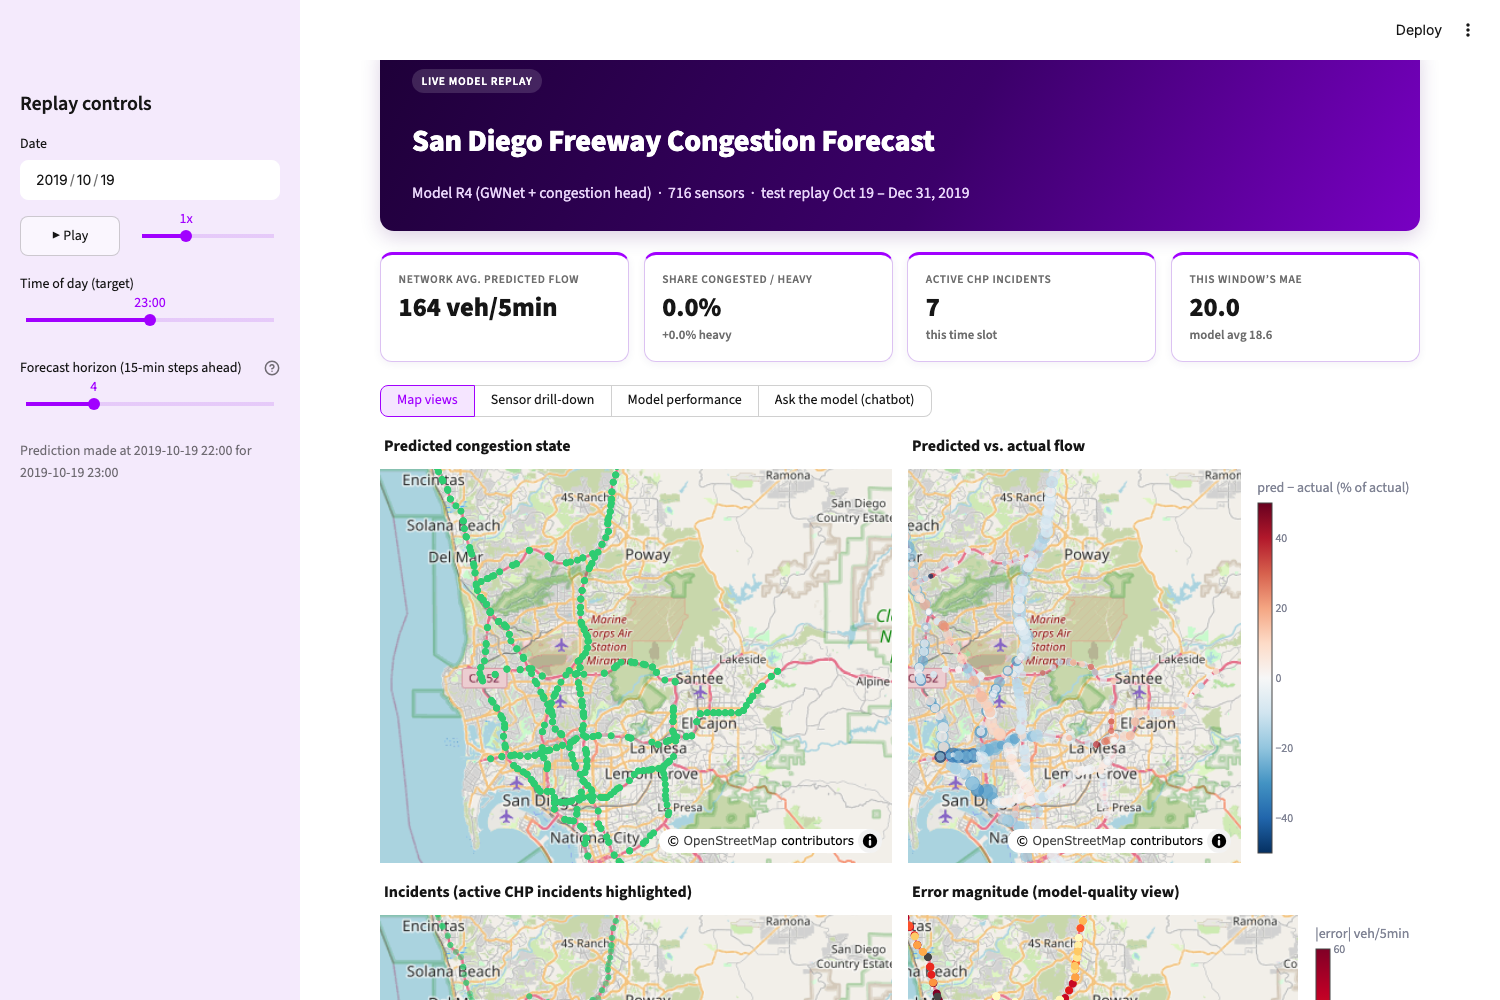
\includegraphics[width=0.92\linewidth]{dashboard_overview.png}
\caption{The dashboard's Map views, showing the hero banner, live KPI row, and the four
synchronized map blocks -- Accenture purple (\texttt{\#A100FF}) governs chrome only, never the
traffic-domain semantic colors (free/heavy/congested) in the maps themselves.}
\end{figure}

\subsection{Agentic chatbot architecture}
The chatbot was originally scoped against the Claude API and, on request, rebuilt against
\textbf{Google Gemini's free tier} -- then deliberately upgraded from basic tool-calling into
something that reads as genuinely agentic: visible reasoning, autonomous multi-step
investigation, an ability to \emph{act} on the dashboard rather than only describe it, and a
self-check before presenting an answer.

\begin{figure}[htbp]
\centering
\resizebox{0.95\linewidth}{!}{%
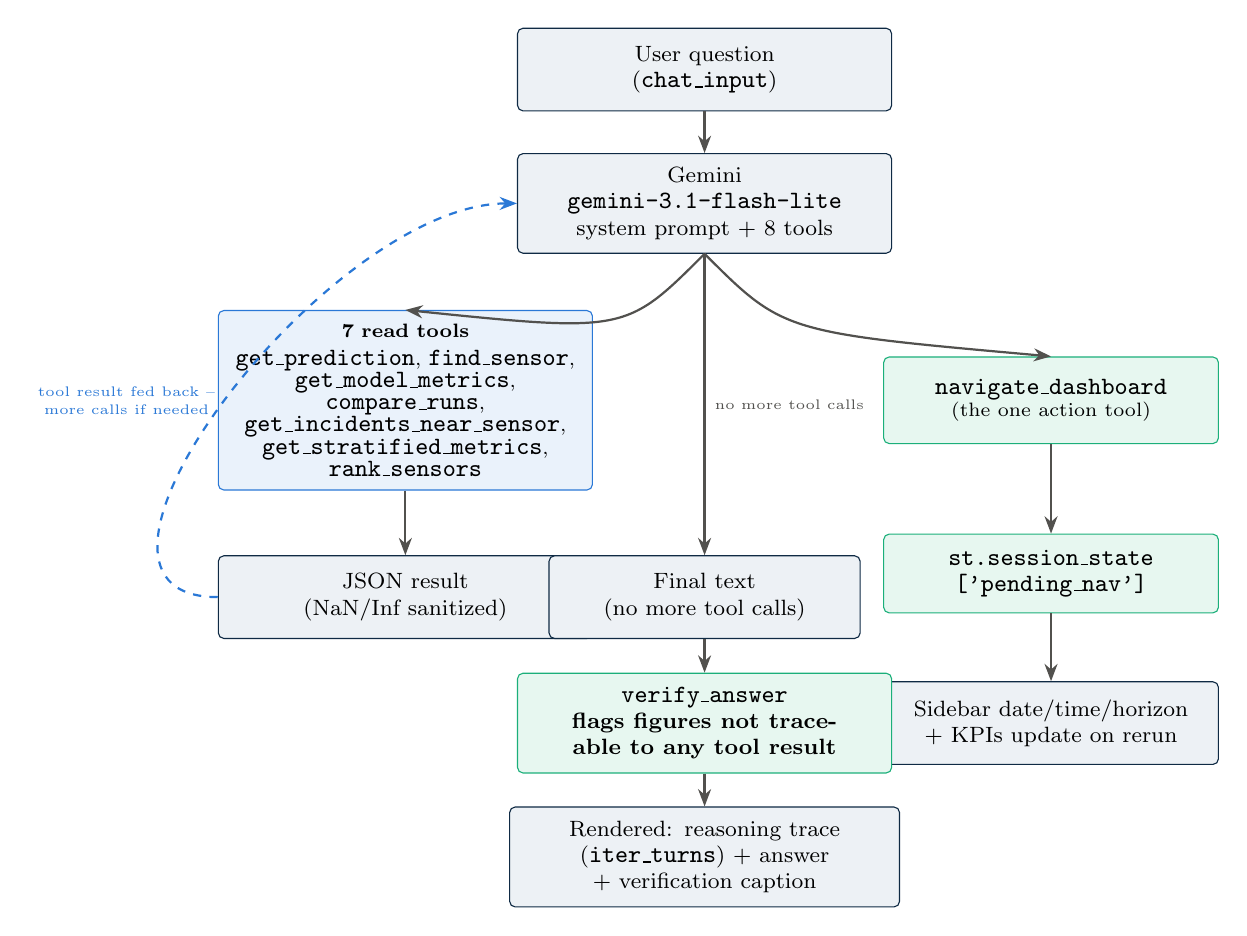
\begin{tikzpicture}[
  main/.style={draw=navy, fill=navyfill, rounded corners=2pt, text width=4.4cm, align=center, font=\footnotesize\headingfont, minimum height=1.05cm, inner sep=5pt},
  tool/.style={draw=steel, fill=steel!10, rounded corners=2pt, text width=4.4cm, align=center, font=\scriptsize\headingfont, minimum height=1.7cm, inner sep=5pt},
  action/.style={draw=accent, fill=accentfill, rounded corners=2pt, text width=3.9cm, align=center, font=\scriptsize\headingfont, minimum height=1.1cm, inner sep=5pt},
  outbox/.style={draw=accent, fill=accentfill, rounded corners=2pt, text width=4.4cm, align=center, font=\footnotesize\headingfont\bfseries, minimum height=1.0cm, inner sep=5pt},
  arr/.style={-{Stealth[length=2.2mm]}, draw=ink2, thick},
  loopback/.style={-{Stealth[length=2.2mm]}, draw=steel, thick, dashed},
]
\node[main] (user) at (0,11.3) {User question\\(\code{chat\_input})};
\node[main] (model) at (0,9.6) {Gemini \code{gemini-3.1-flash-lite}\\system prompt + 8 tools};
\node[tool] (read) at (-3.8,7.1) {\textbf{7 read tools}\\[2pt] \code{get\_prediction}, \code{find\_sensor}, \code{get\_model\_metrics}, \code{compare\_runs}, \code{get\_incidents\_near\_sensor}, \code{get\_stratified\_metrics}, \code{rank\_sensors}};
\node[action] (nav) at (4.4,7.1) {\code{navigate\_dashboard}\\(the one action tool)};
\node[main, text width=4.4cm] (result) at (-3.8,4.6) {JSON result\\(NaN/Inf sanitized)};
\node[outbox, text width=3.9cm] (pending) at (4.4,4.9) {\code{st.session\_state}\\\code{['pending\_nav']}};
\node[main, text width=3.9cm] (sidebar) at (4.4,3.0) {Sidebar date/time/horizon\\+ KPIs update on rerun};
\node[main, text width=3.6cm] (final) at (0,4.6) {Final text\\(no more tool calls)};
\node[outbox] (verify) at (0,3.0) {\code{verify\_answer}\\flags figures not traceable to any tool result};
\node[main, text width=4.6cm] (rendered) at (0,1.3) {Rendered: reasoning trace (\code{iter\_turns}) + answer + verification caption};

\draw[arr] (user) -- (model);
\draw[arr] (model.south) .. controls +(-1,-1) .. (read.north);
\draw[arr] (model.south) .. controls +(1,-1) .. (nav.north);
\draw[arr] (model) -- (final) node[midway, right, font=\tiny\headingfont, text=ink2] {no more tool calls};
\draw[arr] (read) -- (result);
\draw[arr] (nav) -- (pending);
\draw[arr] (pending) -- (sidebar);
\draw[loopback] (result.west) .. controls +(-2.4,0) and +(-2.4,0) .. (model.west)
  node[midway, left, font=\tiny\headingfont, text=steel] {\shortstack{tool result fed back --\\more calls if needed}};
\draw[arr] (final) -- (verify);
\draw[arr] (verify) -- (rendered);
\end{tikzpicture}%
}
\caption{The agentic tool-use loop behind the chatbot. \code{navigate\_dashboard} is the only tool
with a side effect beyond returning data -- it is what lets the agent act on the dashboard rather
than only describe it. The dashed steel arrow is the loop: up to 8 rounds of tool calls can chain
before the model produces a final answer.}
\label{fig:agentic}
\end{figure}

\begin{figure}[htbp]
\centering
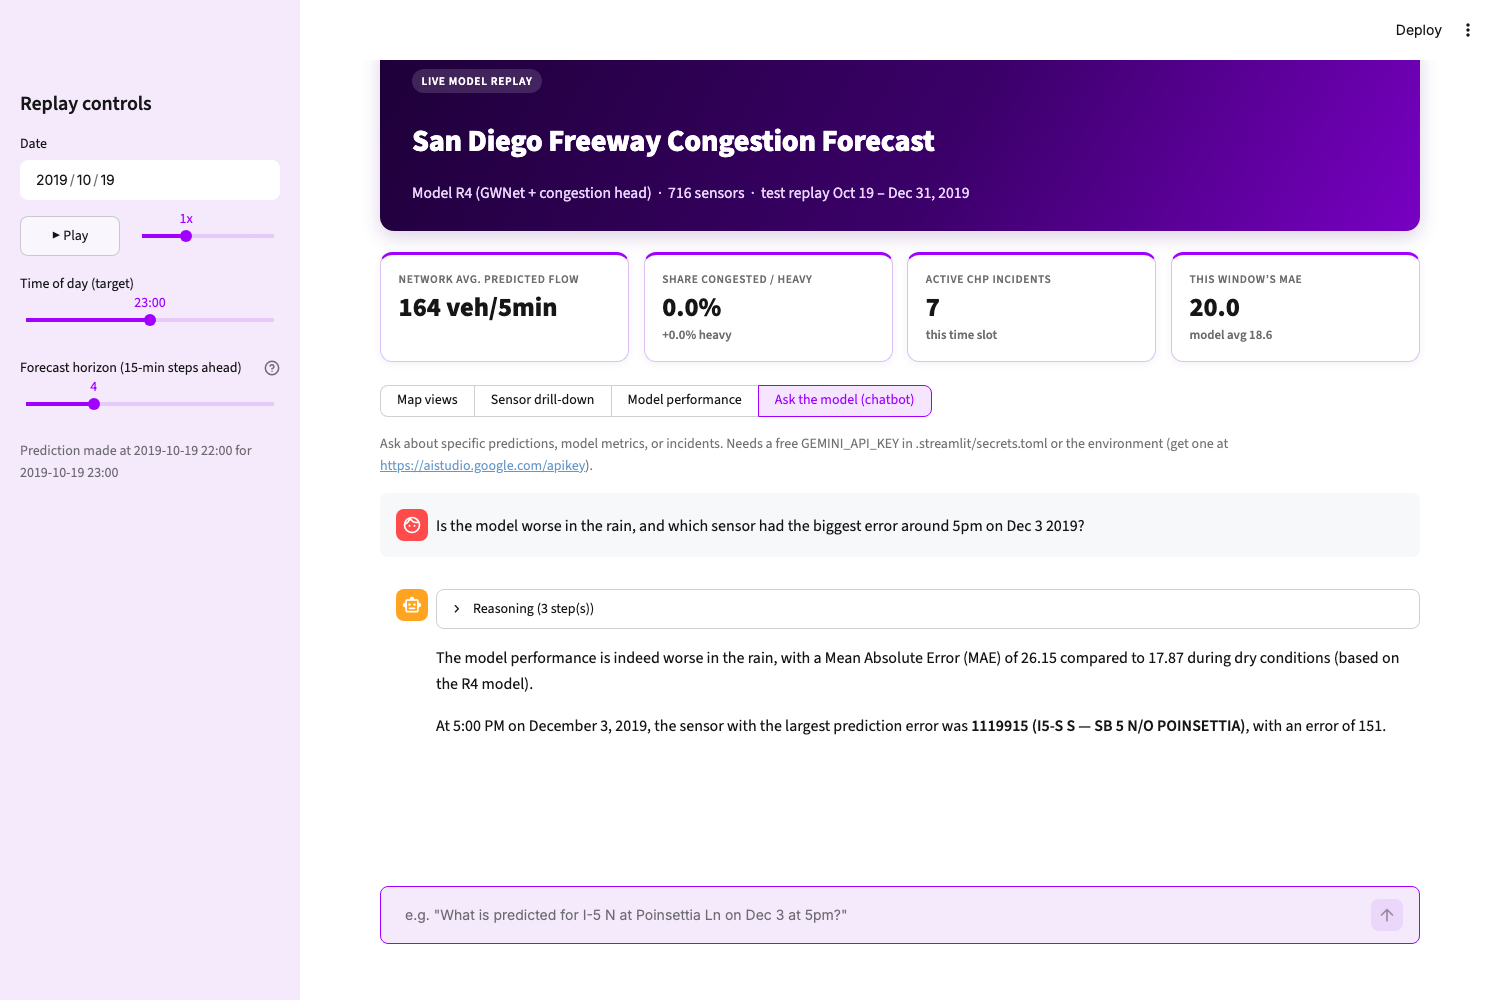
\includegraphics[width=0.92\linewidth]{dashboard_chatbot.png}
\caption{A compound question chaining two tools (\code{get\_stratified\_metrics} for the rain/dry
comparison, \code{rank\_sensors} for the worst-error sensor) in one turn, with the reasoning trace
collapsed and no unverified-figures warning -- every number in the answer traces back to a tool
result.}
\end{figure}

\begin{itemize}
\item \textbf{Eight tools, not five} -- two additions specifically enable the autonomous
  multi-step investigation in Figure~\ref{fig:agentic}: \code{get\_stratified\_metrics} exposes
  the rain/incident/peak/holiday breakdown computed for Gate E (Section~11) but never reachable
  via chat before; \code{rank\_sensors} ranks all 716 sensors at any arbitrary time by congestion,
  error, or flow, not just the dashboard's currently-displayed slice.
\item \textbf{One action tool.} \code{navigate\_dashboard} validates the requested time against
  the test window, then writes \code{st.session\_state['pending\_nav']}, which the dashboard
  resolves into the sidebar's date/time/horizon on the next render -- the one tool whose dispatch
  function has a side effect beyond returning data.
\item \textbf{A visible reasoning trace.} \code{chatbot.iter\_turns()} derives a per-turn
  \code{\{steps, text\}} grouping purely from the existing conversation history at render time (no
  separate bookkeeping structure, to avoid an entire class of state-desync bug), rendered as an
  expandable panel listing every tool call, its arguments, and its result before the final answer.
\item \textbf{A zero-extra-API-call self-check.} \code{verify\_answer} flattens every numeric
  value out of the turn's tool results into a ``known good'' set, regex-extracts candidate numbers
  from the final answer text (explicitly excluding ISO/natural-language dates, clock times,
  7-digit sensor IDs, bare years, and route mentions like ``I-15''/``163 Merge''), and flags
  anything that does not approximately match. Deliberately programmatic, not a second LLM call, to
  protect the free-tier quota -- with the accepted limitation that correct arithmetic the model
  derives from two tool values is flagged too, since only literal tool-returned values count as
  ground truth.
\end{itemize}

\begin{sowhat}
Model choice materially affects reliability on the free tier. The newest model generation
available at build time carried a 20-requests-per-day free quota -- easy to exhaust during
ordinary development, and it fails in a misleading way (an intermittent-looking ``high demand''
error appears before the real quota-exceeded error does). The chatbot instead uses an older, more
generously quota'd tier (\code{gemini-3.1-flash-lite}).
\end{sowhat}

\subsection{Bugs found and fixed}
Four real bugs surfaced only through actually driving the live app -- none were caught by
\code{streamlit.testing.v1.\allowbreak AppTest} alone, which is necessary but not sufficient for
this kind of UI.

\begin{enumerate}
\item \textbf{Chat input unclickable, Safari-only.} \code{st.chat\_input} has documented
  cross-browser bugs when nested inside \code{st.tabs()} (streamlit/streamlit issues \#7814,
  \#8564) -- visible but unresponsive to clicks/focus in some engines. Confirmed Safari-specific
  (worked in Chromium) by testing both browsers on the same machine.
\item \textbf{A \code{400 INVALID\_ARGUMENT} crash from the Gemini API} on a
  \code{rank\_sensors}-triggering question. That tool returns \code{NaN} for sensors with no
  actual reading (LargeST's missing-data sentinel); the first-attempt guard
  (\code{df.where(df.notna(), None)}) does not work -- pandas silently reverts \code{None} back to
  \code{NaN} when assigned into a float64 column. Python's own \code{json.dumps} tolerates the
  resulting NaN (a non-standard literal token, allowed by default), so it never crashed locally --
  but Gemini's own JSON parser is strict and rejects the literal \code{NaN} token once it reaches
  the actual HTTP request. Fixed with a recursive sanitizer applied to \emph{every} tool's result.
\item \textbf{The self-check flagging real sensor names as ``unverified figures.''} PeMS station
  names embed route numbers in free text (``15 SB N/O Carrol Cyn'', ``NB15 @ 163 Merge'')
  indistinguishable by regex alone from real metrics. Fixed by stripping any exact string the tool
  results themselves returned (sensor labels are ``known good'' by construction) plus a
  route-number regex backstop.
\item \textbf{Moving \code{chat\_input} to the top level (the Safari fix) made the entire app
  auto-scroll to the bottom on every load.} On the installed Streamlit version (1.64), a top-level
  \code{chat\_input} anywhere in the script triggers \code{stAppScrollToBottomContainer} for the
  whole page, not just the chat area -- the dashboard would open on ``Ops Watchlist'' instead of
  the hero/KPI row. Root cause: \code{st.tabs()} runs (and mounts in the DOM) every tab's code on
  every rerun regardless of which is visually selected, which is what caused both this and bug 1.
  \textbf{Fix: replaced \code{st.tabs()} entirely with \code{st.segmented\_control()} and plain
  \code{if/elif} blocks} -- a plain \code{if/elif} is not a Streamlit container at all, so only
  the selected view's widgets are ever mounted, eliminating both bugs from one structural change.
\end{enumerate}

\textbf{Verification performed} (not just ``it compiles''): every \code{data.py}/\code{map\_view.py}/
\code{chatbot.py} function was called directly against the real R4 cache and checked against known
numbers; a full \code{AppTest} run hit zero exceptions across every view; and -- because the bugs
above specifically do not show up that way -- a real running server was driven with a headless
browser (and, for the Safari-specific bug, the user's own browser) through compound tool-chaining
questions, a dashboard-navigation command, and a full view-switch-and-back, confirming the
reasoning trace, the verification caption, the KPI updates, and the page's scroll position all
behave correctly together.

% =========================================================================
\section{Reproducibility and Handover}

\begin{enumerate}
\item Download the LargeST San Diego files from LargeST's own release into
  \code{data/traffic/sd\_2019/}.
\item Run \code{congestion\_sd.ipynb} top to bottom, respecting its own gate markers -- the
  notebook was built and executed exactly that way, one gate at a time, not all at once.
\item Download PeMS D11 station and incident files manually and run \code{pems\_filter.py}
  before the labeling and incident-matching stages.
\item Train the nine ablation/graph runs via \code{work/cong/train.py} (or the notebook's own
  training cells) on the recipe in Section~9.
\item Run \code{scripts/export\_predictions.py R4} to build the dashboard's prediction cache.
\item Install dashboard dependencies, add a free Gemini API key, and run
  \code{streamlit run dashboard/app.py}.
\end{enumerate}

% =========================================================================
\section{Status and Roadmap}

\begin{figure}[htbp]
\centering
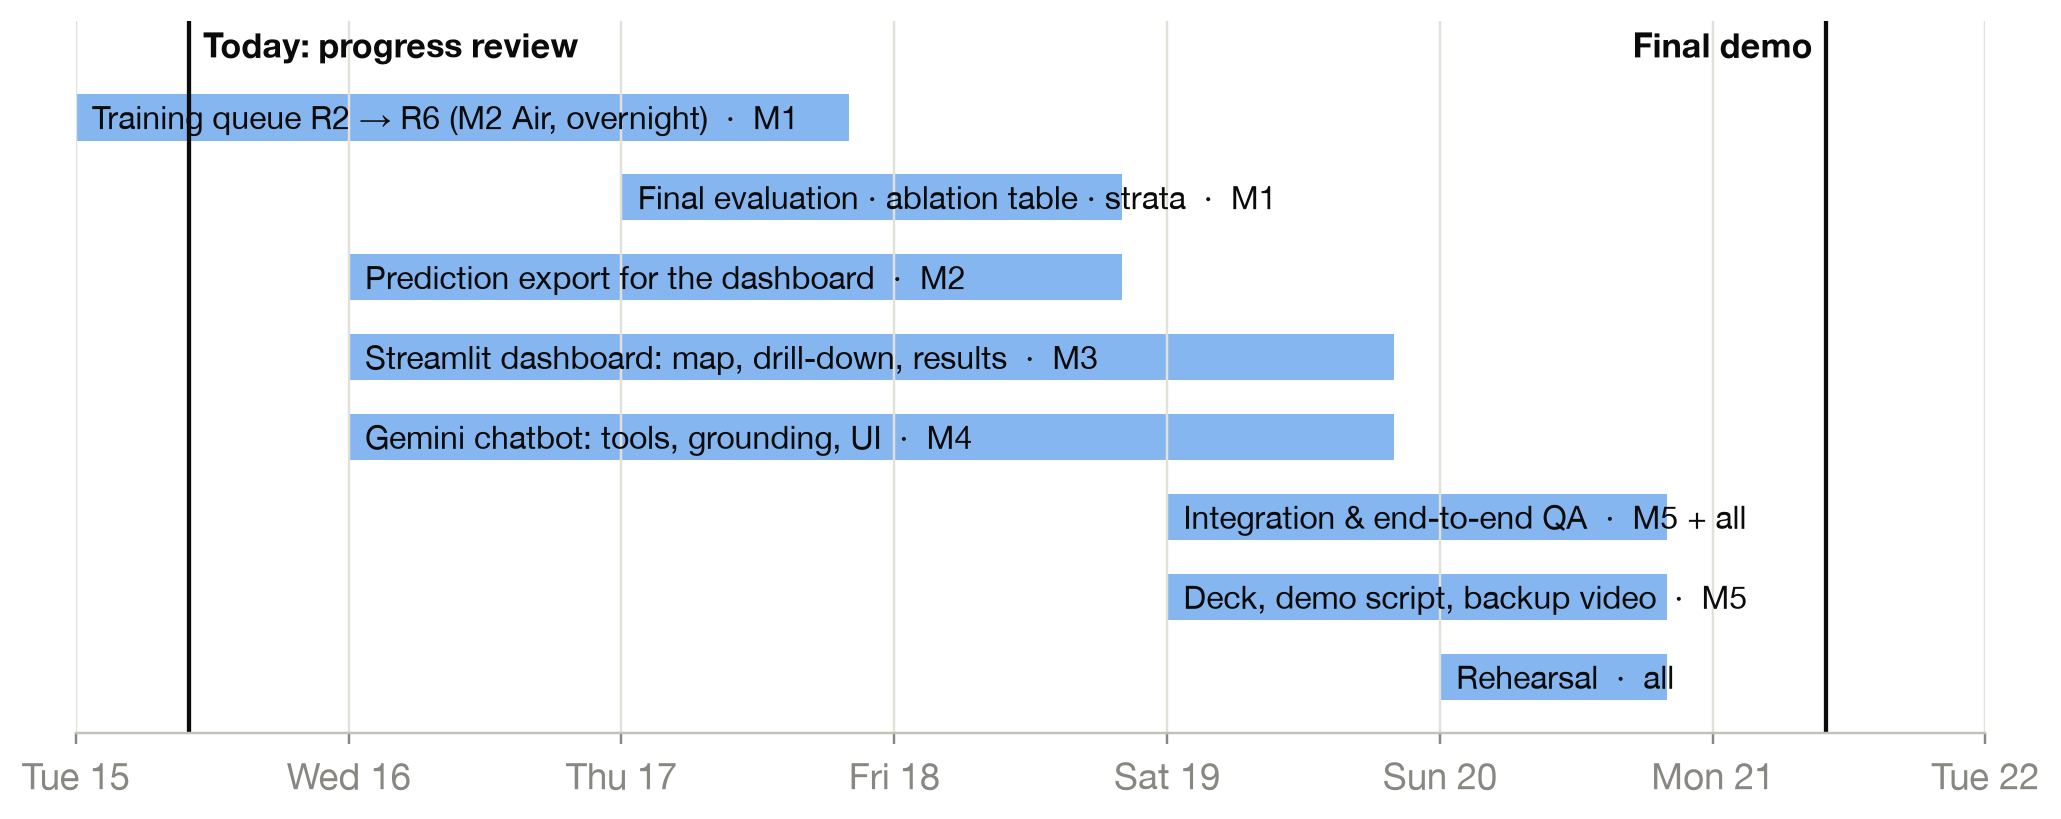
\includegraphics[width=\linewidth]{gantt.png}
\caption{Delivery timeline from the September 15 progress review to the September 21 final demo.}
\end{figure}

\textbf{Complete}: Gates 0/0b/1/2/3, Stage L, Stage I, Stage F, all nine training runs, Gate E, and
a verified local dashboard with an agentic chatbot (8-tool chaining, a visible reasoning trace, a
dashboard-navigation action, and a self-check -- Section~14).

\textbf{Open}: the progress-review deck predates R3--R6, Gate E, and the dashboard's redesign, and
needs updating with the numbers in this report ahead of the September 21 final review.

\end{document}
